\RequirePackage[l2tabu,orthodox]{nag}

% TODO: decide if one-sided/two-sided
%\documentclass[headsepline,footsepline,footinclude=false,fontsize=11pt,paper=a4,listof=totoc,bibliography=totoc,BCOR=12mm,DIV=12]{scrbook} % two-sided % original source stated: BCOR=12mm,DIV=12
\documentclass[headsepline,footsepline,footinclude=false,oneside,fontsize=11pt,paper=a4,listof=totoc,bibliography=totoc,DIV=12]{scrbook} % one-sided

% TODO: change citation style in settings
\PassOptionsToPackage{table,svgnames,dvipsnames}{xcolor}

\usepackage[utf8]{inputenc}
\usepackage[T1]{fontenc}
\usepackage[sc]{mathpazo}
\usepackage[ngerman,english]{babel} % english is the same as american or USenglish
\usepackage[autostyle]{csquotes}
\usepackage[%
  backend=biber,
  url=true,
  style=numeric, % alphabetic, numeric
  sorting=none, % default == nty, https://tex.stackexchange.com/questions/51434/biblatex-citation-order
  maxnames=4,
  minnames=3,
  maxbibnames=99,
  giveninits,
  uniquename=init,
  style=numeric-comp]{biblatex} % TODO: adapt citation style
\usepackage{graphicx}
\usepackage{scrhack} % necessary for listings package
\usepackage{listings}
\usepackage{lstautogobble}
\usepackage{tikz}
\usepackage{pgfplots}
\usepackage{pgfplotstable}
\usepackage{booktabs} % for better looking table creations, but bad with vertical lines by design (package creator despises vertical lines)
\usepackage[final]{microtype}
\usepackage{caption}
\usepackage[hidelinks]{hyperref} % hidelinks removes colored boxes around references and links
\usepackage{ifthen} % for comparison of the current language and changing of the thesis layout
\usepackage{pdftexcmds} % string compare to work with all engines
\usepackage{paralist} % for condensed enumerations or lists
\usepackage{subfig} % for having figures side by side
\usepackage{siunitx} % for physical accurate units and other numerical presentations
\usepackage{multirow} % makes it possible to have bigger cells over multiple rows in a table
\usepackage{array} % different options for table cell orientation
\usepackage{makecell} % allows nice manual configuration of cells with linebreaks in \thead and \makecell with alignments
\usepackage{pdfpages} % for including multiple pages of pdfs
\usepackage{adjustbox} % can center content wider than the \textwidth
\usepackage{tablefootnote} % for footnotes in tables as \tablefootnote
\usepackage{threeparttable} % another way to add footnotes as \tablenotes with \item [x] <your footnote> after setting \tnote{x} 


% https://tex.stackexchange.com/questions/42619/x-mark-to-match-checkmark
\usepackage{amssymb}% http://ctan.org/pkg/amssymb
\usepackage{pifont}% http://ctan.org/pkg/pifont
\newcommand{\cmark}{\ding{51}}%
\newcommand{\xmark}{\ding{55}}%


\usepackage[acronym,xindy,toc]{glossaries} % TODO: include "acronym" if glossary and acronym should be separated
\makeglossaries
\loadglsentries{pages/glossary.tex} % important update for glossaries, before document


\bibliography{bibliography}

\setkomafont{disposition}{\normalfont\bfseries} % use serif font for headings
\linespread{1.05} % adjust line spread for mathpazo font

% Add table of contents to PDF bookmarks
\BeforeTOCHead[toc]{{\cleardoublepage\pdfbookmark[0]{\contentsname}{toc}}}

% Define TUM corporate design colors
% Taken from http://portal.mytum.de/corporatedesign/index_print/vorlagen/index_farben
\definecolor{TUMBlue}{HTML}{0065BD}
\definecolor{TUMSecondaryBlue}{HTML}{005293}
\definecolor{TUMSecondaryBlue2}{HTML}{003359}
\definecolor{TUMBlack}{HTML}{000000}
\definecolor{TUMWhite}{HTML}{FFFFFF}
\definecolor{TUMDarkGray}{HTML}{333333}
\definecolor{TUMGray}{HTML}{808080}
\definecolor{TUMLightGray}{HTML}{CCCCC6}
\definecolor{TUMAccentGray}{HTML}{DAD7CB}
\definecolor{TUMAccentOrange}{HTML}{E37222}
\definecolor{TUMAccentGreen}{HTML}{A2AD00}
\definecolor{TUMAccentLightBlue}{HTML}{98C6EA}
\definecolor{TUMAccentBlue}{HTML}{64A0C8}

% Settings for pgfplots
\pgfplotsset{compat=newest}
\pgfplotsset{
  % For available color names, see http://www.latextemplates.com/svgnames-colors
  cycle list={TUMBlue\\TUMAccentOrange\\TUMAccentGreen\\TUMSecondaryBlue2\\TUMDarkGray\\},
}

% Settings for lstlistings

% Use this for basic highlighting
\lstset{%
  basicstyle=\ttfamily,
  columns=fullflexible,
  autogobble,
  keywordstyle=\bfseries\color{TUMBlue},
  stringstyle=\color{TUMAccentGreen}
}

% use this for C# highlighting
% %\setmonofont{Consolas} %to be used with XeLaTeX or LuaLaTeX
% \definecolor{bluekeywords}{rgb}{0,0,1}
% \definecolor{greencomments}{rgb}{0,0.5,0}
% \definecolor{redstrings}{rgb}{0.64,0.08,0.08}
% \definecolor{xmlcomments}{rgb}{0.5,0.5,0.5}
% \definecolor{types}{rgb}{0.17,0.57,0.68}

% \lstset{language=[Sharp]C,
% captionpos=b,
% %numbers=left, % numbering
% %numberstyle=\tiny, % small row numbers
% frame=lines, % above and underneath of listings is a line
% showspaces=false,
% showtabs=false,
% breaklines=true,
% showstringspaces=false,
% breakatwhitespace=true,
% escapeinside={(*@}{@*)},
% commentstyle=\color{greencomments},
% morekeywords={partial, var, value, get, set},
% keywordstyle=\color{bluekeywords},
% stringstyle=\color{redstrings},
% basicstyle=\ttfamily\small,
% }

% Settings for search order of pictures
\graphicspath{
    {logos/}
    {figures/}
}

% Set up hyphenation rules for the language package when mistakes happen
\babelhyphenation[english]{
an-oth-er
ex-am-ple
}

% Decide between
%\newcommand{\todo}[1]{\textbf{\textsc{\textcolor{TUMAccentOrange}{(TODO: #1)}}}} % for one paragraph, otherwise error!
%\newcommand{\done}[1]{\textit{\textsc{\textcolor{TUMAccentBlue}{(Done: #1)}}}} % for one paragraph, otherwise error!
% and
\newcommand{\todo}[1]{{\bfseries{\scshape{\color{TUMAccentOrange}[(TODO: #1)]}}}} % for multiple paragraphs
\newcommand{\done}[1]{{\itshape{\scshape{\color{TUMAccentBlue}[(Done: #1)]}}}} % for multiple paragraphs
% for error handling of intended behavior in your latex documents.

\newcommand{\tabitem}{~~\llap{\textbullet}~~}

\newcolumntype{P}[1]{>{\centering\arraybackslash}p{#1}} % for horizontal alignment with limited column width
\newcolumntype{M}[1]{>{\centering\arraybackslash}m{#1}} % for horizontal and vertical alignment with limited column width
\newcolumntype{L}[1]{>{\raggedright\arraybackslash}m{#1}} % for vertical alignment left with limited column width
\newcolumntype{R}[1]{>{\raggedleft\arraybackslash}m{#1}} % for vertical alignment right with limited column width

\usepackage{mathtools}
\usepackage{mathalfa}
\usepackage{subfig}
\usepackage{tikz}
\usetikzlibrary{quantikz}
\usepackage{amsthm}
\usepackage{bm}
% \DeclarePairedDelimiter\bra{\langle}{\rvert}
% \DeclarePairedDelimiter\ket{\lvert}{\rangle}
% \DeclarePairedDelimiterX\braket[2]{\langle}{\rangle}{#1 \delimsize\vert #2}
\DeclarePairedDelimiterX\set[1]\lbrace\rbrace{\def\given{\;\delimsize\vert\;}#1}

% TODO: change thesis information
\newcommand*{\getUniversity}{Technische Universität München}
\newcommand*{\getFaculty}{Department of Informatics}
\newcommand*{\getTitle}{Quantum and Classical Generative Modeling for Quantum States Preparation}
\newcommand*{\getTitleGer}{Quantenbasierte und klassische generative Modellierung zur Erzeugung von Quantenzuständen}
\newcommand*{\getAuthor}{Wiktor Jurasz}
\newcommand*{\getDoctype}{Master's Thesis in Quantum Computing}
\newcommand*{\getSupervisor}{Prof. Dr. Christian Mendl}
\newcommand*{\getSubmissionDate}{15.07.2021}
\newcommand*{\getSubmissionLocation}{Munich}

\newcommand{\norm}[1]{\left\lVert#1\right\rVert}
\theoremstyle{definition}
\newtheorem{definition}{Definition}[section]

\begin{document}

% TODO: decide on used language
%\selectlanguage{ngerman}
\selectlanguage{english}

% Set page numbering to avoid "destination with the same identifier has been already used" warning for cover page.
% (see https://en.wikibooks.org/wiki/LaTeX/Hyperlinks#Problems_with_Links_and_Pages).
\pagenumbering{alph}
\begin{titlepage}
  % HACK for two-sided documents: ignore binding correction for cover page.
  % Adapted from Markus Kohm's KOMA-Script titlepage=firstiscover handling.
  % See http://mirrors.ctan.org/macros/latex/contrib/koma-script/scrkernel-title.dtx,
  % \maketitle macro.
  \oddsidemargin=\evensidemargin\relax
  \textwidth=\dimexpr\paperwidth-2\evensidemargin-2in\relax
  \hsize=\textwidth\relax

  \centering

  \IfFileExists{logos/tum.pdf}{%
    
\includegraphics[height=20mm]{logos/tum.pdf}
  }{%
    \vspace*{20mm}
  }

  \vspace{5mm}
  {\huge\MakeUppercase{\getFaculty{}}}\\

  \vspace{5mm}
  {\large\MakeUppercase{\getUniversity{}}}\\

  \vspace{20mm}
  {\Large \getDoctype{}}

  \vspace{15mm}
  \makeatletter
  \ifthenelse{\pdf@strcmp{\languagename}{english}=0}
  {\huge\bfseries \getTitle{}}
  {\huge\bfseries \getTitleGer{}}
  \makeatother

  \vspace{15mm}
  {\LARGE \getAuthor{}}

  \IfFileExists{logos/faculty.png}{%
    \vfill{}
    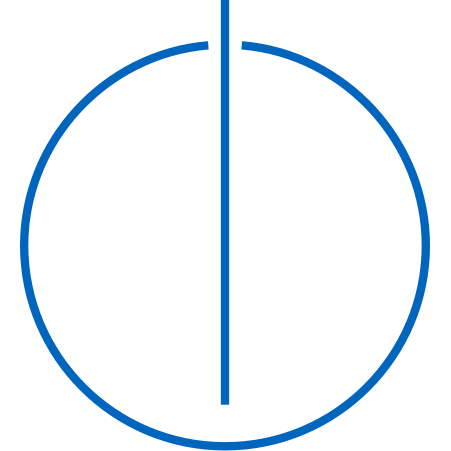
\includegraphics[height=20mm]{logos/faculty.png}
  }{}
\end{titlepage}


\frontmatter{}

\begin{titlepage}
  \centering

  \IfFileExists{logos/tum.pdf}{%
    
\includegraphics[height=20mm]{logos/tum.pdf}
  }{%
    \vspace*{20mm}
  }

  \vspace{5mm}
  {\huge\MakeUppercase{\getFaculty{}}}\\

  \vspace{5mm}
  {\large\MakeUppercase{\getUniversity{}}}\\

  \vspace{20mm}
  {\Large \getDoctype{}}

  \makeatletter
  \vspace{15mm}
  \ifthenelse{\pdf@strcmp{\languagename}{english}=0}
  {
  {\huge\bfseries \getTitle{}}

  \vspace{10mm}
  {\huge\bfseries \foreignlanguage{ngerman}{\getTitleGer{}}}
  }
  {
  {\huge\bfseries \getTitleGer{}}

  \vspace{10mm}
  {\huge\bfseries \foreignlanguage{english}{\getTitle{}}}
  }
  \makeatother

  \vspace{15mm}
  \begin{tabular}{l l}
    Author:          & \getAuthor{} \\
    Supervisor:      & \getSupervisor{} \\
    % Advisor:         & \getAdvisor{} \\
    Submission Date: & \getSubmissionDate{} \\
  \end{tabular}

  \IfFileExists{logos/faculty.png}{%
    \vfill{}
    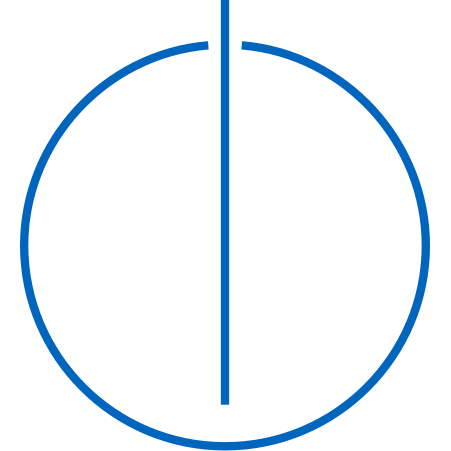
\includegraphics[height=20mm]{logos/faculty.png}
  }{}
\end{titlepage}

\cleardoublepage{}

\thispagestyle{empty}
\vspace*{0.8\textheight}
\noindent
\makeatletter
\ifthenelse{\pdf@strcmp{\languagename}{english}=0}
{I confirm that this \MakeLowercase{\getDoctype{}} is my own work and I have documented all sources and material used.}
{Ich versichere, dass ich diese \getDoctype{} selbstständig verfasst und nur die angegebenen Quellen und Hilfsmittel verwendet habe.}
\makeatother

\vspace{15mm}
\noindent
\getSubmissionLocation{}, \getSubmissionDate{} \hspace{50mm} \getAuthor{}

\cleardoublepage{}

\makeatletter
\ifthenelse{\pdf@strcmp{\languagename}{english}=0}
{\addcontentsline{toc}{chapter}{Acknowledgments}}
{\addcontentsline{toc}{chapter}{Danksagungen}}
\makeatother
\thispagestyle{empty}

\vspace*{20mm}

\begin{center}
\makeatletter
\ifthenelse{\pdf@strcmp{\languagename}{english}=0}
{\usekomafont{section} Acknowledgments}
{\usekomafont{section} Danksagungen}
\makeatother
\end{center}

\vspace{10mm}

%TODO: Acknowledgments

\cleardoublepage{}
 % TODO: if you don't have anyone to thank for or don't wish to publish it, comment this line out.
\chapter{\abstractname}

Generative models and in particular Generative Adversarial Networks (GANs) have
become very popular and powerful data generation tool. In recent years, a major
progress has been made in extending this concept into the quantum realm. In this
work we take a closer look at two different approaches to quantum GANs. We show how they can
be used to learn and generate quantum states, that were supplied in the 
input set and seen at the training time. We also propose a
new quantum-classical hybrid method, that overcomes the limitation of
the current approaches. It allows instead to learn the distribution of the supplied
states and generate new states, that were not a part the input set, but come
from the learned distribution. We
conduct numerous numerical experiments showing, how quantum 
GANs and our method perform on different types of input states and with different
architectures. 






%\makeatletter
%\ifthenelse{\pdf@strcmp{\languagename}{english}=0}
%{\renewcommand{\abstractname}{Kurzfassung}}
%{\renewcommand{\abstractname}{Abstract}}
%\makeatother
%
%\chapter{\abstractname}
%
%%TODO: Abstract in other language
%\begin{otherlanguage}{ngerman} % TODO: select other language, either ngerman or english !
%
%\end{otherlanguage}
%
%
%% Undo the name switch
%\makeatletter
%\ifthenelse{\pdf@strcmp{\languagename}{english}=0}
%{\renewcommand{\abstractname}{Abstract}}
%{\renewcommand{\abstractname}{Kurzfassung}}
%\makeatother
\microtypesetup{protrusion=false}
\tableofcontents{}
\microtypesetup{protrusion=true}

\mainmatter{}

\chapter{Introduction} \label{chapter:introduction}
\section{Problem Statement}
Generative Modeling aims to learn a conditional probability $P(X|Z = z)$, where
$X$ is some observable variable and $Z$ is a target variable. With the knowledge
of this conditional probability, it is possible to generate a new observations $\bar{x} \in X$. In general case, one would not try to obtain the probability $P(X|Z)$ exactly, but learn an approximation. To do so a set of samples $x \in X$ is necessary to train a generator function $G: Z \to X$ which given a target variable $z \in Z$ generates new observation $\bar{x} \in X$. 

In the generative framework, the variable $X$ is a multidimensional vector, in particular it can be used to describe an arbitrary quantum state. With this setup, given a finite set of quantum states $\mathcal{Q} = \set{\ket{\psi_i}}, \ket{\psi_i} \in X\; \forall_i$ the generator function $G$ prepares a new quantum state $\ket{\hat{\psi}}$. This new quantum state is expected to come from the same distribution as the samples in the input set $\mathcal{Q}$.

The only missing piece in the above description is the target variable $Z$. In
the context of the function $G$ generating the quantum states, we can think
about $Z$ as a label of the generated state. That is, for a specific $z \in Z$
the function $G$ always generates the same $\ket{\hat{\psi}}$.

In this work we evaluate different approaches to find the probability $P(X|Z =
z)$ by learning the function $G$. We also address the limitations of the
existing methods propose a new one that combines quantum and classical
generative modeling.
\section{Previous Work}
There exist many different types of generative models. In this work we focus on
one particular type, namely Generative Adversarial Networks (GANs). First
version of GANs was proposed by Goodfellow et al.
\cite{goodfellow2014generative} (to which we refer as Standard GANs - SGANs),
since then many different variations of GANs were invented
\cite{mirza2014conditional}\cite{karras2019stylebased}\cite{radford2016unsupervised}.
In context of this work, particularly interesting are Wasserstein GANs
(WGANs) \cite{arjovsky2017wasserstein} which minimize the \textit{Earth-Mover} distance
between two probability distribution instead of
\textit{Jensen–Shannon} divergence (see Chapter \ref{chapter:gans}) as in SGANs.

In recent years there has been an increasing interest in realizing Generative
Adversarial Networks in Quantum Computing (QC) realm. Dallaire-Demers et al.
proposed QuGANs \cite{Dallaire_Demers_2018} - Quantum Generative Adversarial Networks
where generator and discriminator are parametrized quantum circuits. Similarly
Benedetti et al. proposed fully quantum GANs for pure state approximation \cite{Benedetti_2019}, but
with different (more suitable for NISQ \cite{Preskill_2018}) learning method.
Hybrid methods were also explored, Zoufal et al. built qGAN \cite{Zoufal_2019} -
with parametrized quantum circuit as the generator and a classical neural network
as the discriminator. 

De Palma et al. proposed quantum equivalent of the Wasserstein distance of order 1
\cite{depalma2020quantum} which made Quantum Wasserstein GANs
(QWGANs) \cite{kiani2021quantum} possible. This variation of quantum GANs
consist of the parametrized quantum circuit as the generator and the classical linear
program as the discriminator.

\section{Our Contribution}
There has been a substantial effort in the direction of bringing GANs into the quantum
realm. Nevertheless, this is still very early stage and many more routs are yet
to be explored. In this work we focus on building quantum GANs that can generate
new, unseen at the training time, quantum states. The majority of the models
proposed so far are only able to generate the states the have 
been a part of the input set and were evaluated at the training time. Only some 
architectures \cite{Dallaire_Demers_2018} account for the random noise in the input
that allows to generate new, unseen states. However, as we discuss later, those are
mostly theoretical and do not seem to work well in practice.


We propose a new quantum-classical hybrid method. First, it learns the
distribution over the expectations of some predefined set of measurements, and later uses this
distribution to generate an unlimited number of unseen quantum states, that were not part of the input
set. We utilize the fully quantum and fully classical generative models that
work together in one framework. 

We proceed as follows. In Chapter \ref{chapter:quantum_mechanic_introduction} we
establish the quantum computing notation used in the reminder of this work. In
Chapter \ref{chapter:gans} we give a general introduction to classical GANs. In
Chapter \ref{chapter:quantum_gans} we combine the knowledge from the previous
chapters to introduce the concept of quantum GANs and talk more about the
different variations of quantum GANs and their limitations. We also evaluate the
performance of quantum GANs on different input types. In Chapter
\ref{chapter:my_contribution} we introduce and describe in depth our
concept of hybrid quantum-classical generative framework and empirically show the
quality of the unseen states generated by the proposed framework. Finally, in Chapter
\ref{chapter:conclusions} we conclude our finding and talk briefly about the
possible future directions. 

%%% Local Variables:
%%% mode: latex
%%% TeX-master: "../main"
%%% End:

\chapter{Quantum Computing Notation}\label{chapter:quantum_mechanic_introduction}
\enlargethispage{\baselineskip}
We use the standard bra-ket notation to represent vectors in complex
$N$-dimensional Hilbert space $\mathbb{C}^N$, i.e.
$\ket{\cdot} \in \mathbb{C}^N$ for column vector and $\bra{\cdot} \in
(\mathbb{C}^{N})^{\dagger}$ for row vector and complex conjugate of
$\ket{\cdot}$.

In this work we operate on quantum states composed of qubits. A single qubit is
represented as a vector $\ket{\psi} \in \mathbb{C}^2$, such that $\ket{\psi} =
\alpha\ket{0} + \beta\ket{1}$, where 
\begin{align*}
  \ket{0} = \begin{pmatrix}
    1 \\
    0 
  \end{pmatrix},\ 
  \ket{1} = \begin{pmatrix}
    0 \\
    1 
  \end{pmatrix},\ 
  |\alpha|^2 + |\beta|^2 = 1,\
  \alpha, \beta \in \mathbb{R}
\end{align*}
We denote a pure quantum state as a tensor product of $n$ qubits, i.e.
$\ket{\psi_1} \otimes \ldots \otimes \ket{\psi_n} = \ket{\psi_1 \ldots \psi_n} =
\ket{\psi}^{\otimes n} \in
\mathbb{C}^{2^n}$. For the simplicity of notation we often write
$\ket{\psi}^{\otimes n} = \ket{\psi}$.

If some system is a mixture of several pure quantum states, we use density
operator to describe it. The density operator $\rho$ is defined as $\rho =
\sum_{i=1}^{k}p_i\ket{\psi_i}\bra{\psi_i}$, where $p_i$ is the probability of
system being in state $\ket{\psi_i}$ and $\sum_{i=1}^kp_i = 1$.

An observable is an Hermitian matrix $H \in \mathbb{C}^{2^n \otimes 2^n}$. We
call $Tr[\rho H]$ the expected value of observable $H$ on state $\rho$, where
$Tr$ is matrix trace operation. Since the quantum state $\rho$ cannot be directly
observed, in practice quantum measurements \cite{10.5555/1972505} are used to
estimate the $Tr[\rho H]$.

An operator, or a quantum gate, is an Unitary matrix $U \in \mathbb{C}^{2^n
  \otimes 2^n}$. The operators are used to describe a transition from one
quantum state to another, i.e. $\ket{\psi'} = U\ket{\psi}$.
Similarly to the quantum states, operators may be stated as a tensor
product of $2 \times 2$ Hermitian matrices, i.e. $H = H_1 \otimes \ldots \otimes
H_n \in \mathbb{C}^{2^n \otimes 2^n}$. For the simplicity of notation we skip the
identity matrices in the tensor product notation, e.g. $H_1 \otimes I \otimes H_3
\otimes I \otimes I \otimes H_6 = H_1 \otimes H_3 \otimes H_6$.

In context of this work, particularly important are 3 Pauli Matrices:
\begin{align*}
  X = \begin{pmatrix}
    0 & 1 \\
    1 & 0 
  \end{pmatrix},\ 
  Y = \begin{pmatrix}
    0 & -i \\
    i & 0 
  \end{pmatrix},\ 
  Z = \begin{pmatrix}
    1 & 0 \\
    0 & -1 
  \end{pmatrix}.
\end{align*}

Those matrices are Hermitian and Unitary, which means they can be used as
observables and operators. We refer to tensor product of several Pauli Matrices
as Pauli String. We also use the Pauli Matrices to define basic parametrized gates
$R_{\sigma}(\theta) = e^{-i\theta \sigma / 2}$, where $\sigma \in \{X, Y, Z\}$
and $\theta \in \mathbb{R}$ is the parameter.
More complex parametrized gates can be build with linear combinations or tensor
products of Pauli Matrices. 

To describe the evolution of quantum state, we use quantum
circuit representation. The operation $\ket{\psi'} = U_k\ldots U_1\ket{\psi}$ is equivalent
to the circuit \ref{fig:small_circuit}.
\begin{figure}[htbp!]
  \centering
  \begin{tikzcd}
    \lstick{$\ket{\psi}$} & \gate{U_1} & \qw & \ldots && \gate{U_k} & \qw && \lstick{\ket{\psi'}}
  \end{tikzcd}
  \label{fig:small_circuit}
\end{figure}
If any of the gates $U$ is parametrized, we call this such circuit a
parametrized quantum circuit. For further details about the notation and quantum
computing in general, please refer to the book \cite{10.5555/1972505}.


%%% Local Variables:
%%% mode: latex
%%% TeX-master: "../main"
%%% End:
\chapter{Generative Adversarial Networks Introduction}\label{chapter:gans}
Generative Adversarial Network (GAN)\cite{goodfellow2014generative} is a
machine learning framework designed to estimate generative models using
adversarial process. At the core it consists of two models: the generative one
$G$ which is capable of learning the distribution of the provided data and
discriminative model $D$ that, given a data point, estimates whether it comes
from input data or was generated by $G$. The models are set to compete with each
other in a minmax game. $D$ is trained to maximize the probability of correctly
distinguishing between the generated and real samples, while $G$ is trained to
minimize it.  

To approximate the true distribution $p_r$ over data $X$ we define a prior noise
distribution $p_z$ over noise input $Z$ and the generator distribution $p_g$
over data $X$. The generator represents a mapping
$G(z \sim Z; \theta_g) \to x \sim X$, where $\theta_g$ is some learnable
parameter (summary in Table \ref{tab:gan_probabilities}).

The discriminator $D(x, \theta_d) \to [0;1]$ is a function that given a sample $x
\sim X$ outputs the probability whether $x$ comes from data or was generated by
$G$. 

In classical GANs both $G$ and $D$ are most often modeled as multi-layer
perceptrons\cite{goodfellow2014generative} or other types of neural networks
(e.g. convolutional neural networks \cite{radford2016unsupervised}). However,
there exist many different variations of cost functions used during the mixmax
training procedure. In the following paragraphs we take a closer look at two of
them, namely SGANs and WGANs, which are the most relevant in the context of this
work. To simply the notation, we skip the $\theta$ parameters, i.e. $G(z,
\theta_g) = G(z)$ and $D(x, \theta_d) = D(x)$
\begin{table}[]
  \centering
  \begin{tabular}{|l|l|}
    \hline
    Probability Distribution & Description  \\ \hline
    $p_z$ & True distribution over noise input $Z$ \\ \hline
    $p_g$&  Approximated distribution over input data $X$ given by $G$ \\ \hline
    $p_r$&  True distribution over input data $X$\\ \hline
  \end{tabular}
  \caption{\label{tab:gan_probabilities} Description of the probability
    distributions used in GANs}
\end{table}

\section{Standard Generative Adversarial Networks (SGANs)}
The goal of $D$ is to distinguish between the real and generated samples. For $x
\sim X$ the output $D(x)$ should approach $1$, while for $x \sim G(z)$ it should
approach $0$. In other terms it simultaneously maximizes $\mathbb{E}_{x \sim
  p_r(x)}[\log{D(x)}]$, and $\mathbb{E}_{z \sim p_z(z)}[\log{1 - D(G(z))}]$.

Generator $G$ has an opposite objective, thus it minimizes the $\mathbb{E}_{z
  \sim p_z(z)}[\log{1 - D(G(z))}]$.

Putting it all together, we get the objective for SGANs \ref{eq:SGANs_objective}.
\begin{equation}
  \label{eq:SGANs_objective}
  \begin{split}
    \min_G\max_D\mathcal{L(G, D)} & = \min_G\max_D \mathbb{E}_{x \sim p_r(x)}[\log{D(x)}] +  \mathbb{E}_{z \sim p_z(z)}[\log{1 - D(G(z))}] \\
    & = \min_G\max_D \mathbb{E}_{x \sim p_r(x)}[\log{D(x)}] +  \mathbb{E}_{x \sim p_g(x)}[\log{1 - D(x)}]
  \end{split}
\end{equation}
It can be shown, that if $D$ is optimal, this loss function measures the similarity between 
$p_r$ and $p_g$ according to Jensen–Shannon divergence (see Appendix
\ref{apx:JSD} for detailed analysis). 

SGANs are a very powerful tool, however, the training process is very difficult
and unstable \cite{salimans2016improved}. Additionally, if the data exists in
low dimensional manifold (which seems to be the case for most real world data
\cite{narayanan2010proceedings}), $p_r$ and $p_g$ are very likely disjoint and we are always capable of finding the perfect discriminator 
\cite{arjovsky2017principled}. This might seem like a good
characteristic, but if we examine the loss function closer, we find that it
makes generator incapable of learning. For the perfect $D$ we have $\forall x
\sim X, D(x) = 1$ and $\forall z \sim Z, D(G(z)) = 0$. For those values
$\mathcal{L(G,D)} = 0$ gradient vanishes and the gradient based optimizers cannot improve the
generator anymore.
\section{Wasserstein Generative Adversarial Networks (WGANs)}
One of the very prominent improvement to SGANs and a way to mitigate the
vanishing gradient problem is changing the cost function to use Wasserstein
Distance.

The Wasserstein Distance, also called Earth-Mover's Distance is a distance
measure between two probability distributions. The name ``Earth Mover'' comes
from the fact, that informally the distance can be described as follows: Given
two probability distributions, if we imagine them as piles of dirt, the ``Earth
Mover'' distance says what is the minimum cost of turning one pile of dirt into the
other one. Where cost is the volume that has to be moved times the distance is
has to be moved.

The main advantage of the Wasserstein Distance over Jensen–Shannon Divergence is,
that even in the case of disjoint distribution we get meaningful, stable
distance which is well suited for gradient based learning.

Formally, the Wasserstein or Earth-Mover's Distance (EM Distance) is defined as
follows:

\begin{equation}
  \label{eq:EMD}
  W(p_r, p_g) = \inf_{\gamma \in \Pi(p_r, p_g)} \mathbb{E}_{(x, y) \sim \gamma}[\norm{x-y}]
\end{equation}

Where $\Pi(p_r, p_g)$ denotes the set of all possible joint distributions,
$\gamma(x,y)$ says how much ``dirt'' has to be transported in order to transform
$p_g$ into $p_r$. Since we take $\inf$, the EM Distance is then the cost of such
transport done in the optimal way. 

The computation in \ref{eq:EMD} is highly intractable, but according to
Kantorovich-Rubinstein duality \cite{villani@optimal}, we can rewrite it as
follows.

\begin{equation}
  \label{eq:EMD2}
  W(p_r, p_g) = \frac{1}{K} \sup_{\norm{f}_L < K} \mathbb{E}_{x \sim p_r}[f(x)] - \mathbb{E}_{x \sim p_g}[f(x)]
\end{equation}

Where the supremum is overall all K-Lipschitz functions $f$. In practice it is
impossible to go over all such functions. Instead we define a family of parameterized
functions $\{f_{w}\}_{w \in W}$ and using the same notation for the generator as
in SGANs the WGANs objective becomes


\begin{equation}
  \label{eq:EMDL}
  \max_{f}\min_{G}\mathcal{L}(f, G) = \max_{f}\min_{G}  \mathbb{E}_{x \sim p_r}[f_w(x)] - \mathbb{E}_{z \sim p_z}[f_w(G_{\theta}(z))]
\end{equation}.

Here the function $f_w$ represents the ``discriminator'', however it does not
anymore tries to distinguish between real and fake samples. Instead it is
trained to to approximate K-continous Lipschitz function and compute the
Wasserstein distance. The one missing part from the Equation \ref{eq:EMDL} is
ensuring the $f_w$ Lipschitz continuity, this can be achieved by gradient
clipping \cite{arjovsky2017wasserstein} or gradient penalty \cite{gulrajani2017improved}.

%%% Local Variables:
%%% mode: latex
%%% TeX-master: "../main"
%%% End:
\chapter{Quantum Generative Adversarial Networks}\label{chapter:quantum_gans}
The field of Quantum Machine Learning (QML) is still in very early stages and there
has been an ongoing effort on translating the  classical Machine Learning (ML)
concepts into QML realm. Because of the limitations of current quantum computers
(NISQ) \cite{bharti2021noisy} and overall different paradigm of Quantum
Computing (QC), this process is difficult and there is no clear
answer to the question ``how this concept should be realized on QC device?''.
While in classical GANs generator and discriminator are realized as deep neural
networks, NISQ devices are not yet powerful enough to support such architecture.
Instead parametric quantum circuits \cite{Schuld_2020} are used.

In this chapter we take a closer look at two different designs of quantum GANs.
We briefly explain theory behind them and show the results of our evaluation.
The quantum GANs introduced in this chapter are the base of our hybrid
classical-quantum generative framework.

\section{Standard Quantum GANs (SQGANs)}
In the classical GANs, both the discriminator and generator are deep, general
purpose neural networks. The logical extension of this design in the quantum
realm is to model those are general purpose parametric quantum circuits. This
idea was formalized by Dallaire-Demers et al. \cite{Dallaire_Demers_2018} in
the architecture we call SQGANs (Figure \ref{fig:SQGANs_circuit}). The generator
starts in the state $\ket{0}^{\otimes n}$ in the \textbf{Our R/G} wire, where
$n$ is the dimension of the real quantum samples.
Additionally, the generator takes the label state $\ket{\lambda}$ in the
\textbf{Label R/G} wire and the random state $\ket{z}$ that provides the entropy in
the \textbf{Batch R/G} wire. The label state $\ket{\lambda}$ lets the
generator to learn the conditional distribution $p_g(x|\lambda)$ instead of $p_g(x)$,
this design was inspired by classical Conditional GANs
\cite{mirza2014conditional}. The discriminator takes the generated state
$\rho_\lambda^G$ or real state $\rho_\lambda^R$ and the corresponding label
$\ket{\lambda}$ in the \textbf{Label D} wire, it also uses the workspace
\textbf{Batch D} initialized in $\ket{0}$ state. The measurement on the single
qubit wire \textbf{Out D} corresponds to the probability of the state in 
\textbf{Out R/G} being real or generated.

There are not any particular restrains on how $G$ and $D$ circuits should look
like. However, to be able to learn and differentiate between arbitrary quantum
states the ansatz used should be universal (i.e. be able to generate every
quantum state given appropriate depth). The ansatz used in this
work is described in details in Appendix \ref{apx:sqgans_ansatz}.

\begin{figure}[htbp!]
  \begin{tikzcd}
    \rstick{Out D} &&&&&& \rstick{$\ket{0}$} &&& \qw & \qw & \gate[4, disable auto height]{D(\theta_D)} & \meter{} \\
    \rstick{Batch D} &&&&&& \rstick{$\ket{0}^{\otimes d}$} &&& \qw & \qw & & \qw \\
    \rstick{Label D} &&&&&& \rstick{$\ket{\lambda}$} &&& \qw & \qw & & \qw \\ 
    \rstick{Out R/G} &&&&&& \rstick{$\ket{0}^{\otimes n}$} &&& \gate[3, disable auto height]{
      \begin{array}{c}
      R \\ or \\ G(\theta_G)
      \end{array}
    } & \qw \rho_{\lambda}^{R/G} & & \qw \\ 
    \rstick{Label R/G} &&&&&& \rstick{$\ket{\lambda}$} &&& \qw & \qw & \qw & \qw \\ 
    \rstick{Batch R/G} &&&&&& \rstick{$\ket{z}$} &&& \qw & \qw & \qw & \qw 
  \end{tikzcd}
  \caption{SQGANs schema. The discriminator $D$ and the generator $G$ are
    parametric quantum circuits. The first 3 wires go
    directly to the discriminator. \textbf{Out D} outputs the probability of the
  input being generated. \textbf{Batch D} is an additional workspace of the
  discriminator and \textbf{Label D} contains the label state. \textbf{Out R/G}
  carries the generated or real state. \textbf{Label R/G} contains the label
  state and \textbf{Batch R/G} is the noise source for the generator, not used
  with the real samples.\label{fig:SQGANs_circuit} }
\end{figure}

\subsection{Training}
As in the SGANs we are interested in the minmax game setting. Specifically, in
the \textbf{Out D} wire, the measurement of $\ket{1}$ indicates that the sample
was real and $\ket{0}$ that the state was generated by $G$.
\footnote{Using $\ket{1}$ and $\ket{0}$ in this order is just a convention we
  assume. Any other orthogonal pair can be used.}
This should be the case for each label state $\ket{\lambda}$, which gives the
objective \ref{eq:SQGANs_objective}. 
\begin{equation}
  \begin{split}
  \label{eq:SQGANs_objective}
  & \max_{D}\min_{G} \mathcal{L}(G, D) = \\
  & \max_{D}\min_{G}  \frac{1}{\Lambda}\sum_{\lambda \in \Lambda}{P((D(\theta_D, \ket{\lambda}, R(\lambda)) = \ket{1}) \land (D(\theta_D, \ket{\lambda}, G(\theta_G, \ket{\lambda}, \ket{z}) = \ket{0})))}
  \end{split}
\end{equation} 
Where the discriminator objective is to maximize the probability of measuring $\ket{1}$
given real sample and measuring $\ket{0}$ given generated state. At the same
time for the generator the objective is to do the opposite.

The SQGANs cost function \ref{eq:SQGANs_objective} in contrast to the SGANs cost
function \ref{eq:SGANs_objective} is not defined with log-likelihood. In quantum
setup is more natural to work with linear functions and since the $\log$ is
convex, the optimum is the same for both.

The cost function $\mathcal{L}(G, D)$ expressed in terms of measurements and
assuming equal probability of sampling from $R$ and $G$ takes the form \ref{eq:SQGANs_objective}

\begin{equation}
  \label{eq:SQGAN_objective_trace}
  \mathcal{L}(G, D) = \frac{1}{2} + \frac{1}{4\Lambda}\sum_{\lambda \in
  \Lambda}{}tr((\rho_\lambda^{DR}(\theta_D) - \rho_\lambda^{DG}(\theta_D, \theta_G, z))Z)
\end{equation}
For detailed derivation on how to get from \ref{eq:SQGANs_objective} to
\ref{eq:SQGANs_objective} refer to Appendix \ref{apx:sqgans_cost_function}.

\subsubsection{Gradient Estimation}
To optimize the parameters $\theta_D$ and $\theta_G$ classical gradient descent
method was used. First, the value of the cost function $\mathcal{L}(G, D)$ was
estimated by sampling from the circuit \ref{fig:SQGANs_circuit}. This allows to
calculate the gradient w.r.t. $\theta_D$ and $\theta_G$ on classical computer
and update the parameters at the step $k$ in the following way
\begin{equation}
  \begin{split}
    \theta^{k+1}_D = \theta^{k}_D + \alpha^k_D\nabla_{\theta_D}\mathcal{L}(\theta^k_G, \theta^k_D) \\
    \theta^{k+1}_G = \theta^{k}_G - \alpha^k_G\nabla_{\theta_G}\mathcal{L}(\theta^k_G, \theta^k_D)
  \end{split}
\end{equation}
where $\alpha^k_D$ and $\alpha^k_G$ are learning rate metaparameters that can
depend on the step $k$.

It is also possible to estimate the gradient directly on quantum computer by
creating an explicit quantum circuit for each element of vectors $\theta_D / \theta_G$
and reading the grading by sampling for those circuits \cite{Dallaire_Demers_2018}.
\subsection{Evaluation Results}
\subsubsection{Experimental Setup}
In all of the experiments the real samples are generated by evaluating the
circuit from Figure \ref{fig:phase_circuit_small}. This circuit was constructed
by Smith et al. \cite{smith2020crossing} to study topological phase transitions.
All the gates in the circuit are parameterized by a single real valued parameter
$g \in [-1;1]$. The detailed gates layout is described in Appendix \ref{apx:topological_phase_transition_ansatz}.
\begin{figure}[htbp!]
  \begin{tikzcd}
    \lstick{$\ket{0}$} & \gate[2, disable auto height]{U_1(g)} & \qw & \qw & \qw &
    \qw & \qw & \qw \\
    \lstick{$\ket{0}$} & & \gate[2, disable auto height]{U(g)}  & \qw & \qw & \qw & \qw & \qw \\
    \lstick{$\ket{0}$} & \qw & \qw & \gate[2, disable auto height]{U(g)}  & \qw & \qw & \qw & \qw \\
    \lstick{$\ket{0}$} & \qw & \qw & \qw & \qw & \ldots  \\
    \vdots & & & & &\ldots & \gate[2, disable auto height]{U(g)} & \qw \\
    \lstick{$\ket{0}$} & \qw & \qw & \qw & \qw & \qw & \qw & \qw \\
  \end{tikzcd}
  \caption{The circuit used for generating real samples. All the gates are
    parametrized by a real valued parameter $g \in [-1; 1]$. For detailed
    description of the circuit see Appendix
    \ref{apx:topological_phase_transition_ansatz} \label{fig:phase_circuit_small}}
\end{figure}

The generator and discriminator are both build using the generic circuit
architecture from Appendix \ref{apx:sqgans_ansatz}. The number of layers differs
and is specified for each experiment separately.

In all the experiment we use Adam optimizer \cite{kingma2017adam} with
parameters $\beta_1 = 0.9$, $\beta_2=0.98$, $\hat{\epsilon} = 1e-9$. The
learning rate is calculated as
\begin{equation}
lr = \max{(\exp{(-\frac{(k+200) * \ln{100}}{4000}), 0.01)}
\end{equation}
where $k$ is the optimization step number. The
learning rate decreases from $\sim 0.8$ to $0.01$ in the first $3800$ steps and then
remains at $0.01$ for the rest of the training. The exact values were derived
experimentally and show overall good convergence. The exact number of epochs and
iterations is specified for each experiment separately.
\subsubsection{Results For Pure State Real Input}
In this setup the generator is fed the same real input state at every iteration.
The real input state is generated using circuit from Figure
\ref{fig:phase_circuit_small} for random $g \in [-1; 1]$.


In Figure \ref{fig:sqgans_res_3} we present the
results of experiments for different widths of the real input circuit. For All
the experiments, the generator and discriminator were built using ansatz
from Appendix \ref{apx:sqgans_ansatz} for each layer. The \textbf{Label} and
\textbf{Batch} wires are not used for any circuit.

For each real input width the generator was able to approximate the real source,
increasing the fidelity as the training progressed. The training was
harder for the bigger real source circuits and it can be clearly seen that
the results for wider inputs are worse. Not only the final fidelity is lower, but
also it fluctuates much more. It is also much harder for the generator to fool
the discriminator for wider inputs.

It is not surprising that it is more difficult to train circuits with more
qubits. We also acknowledge that with different metaparameters or optimization
method the results could be better. However, our best results for more than 5 qubits
in the real source are not longer useful for the real source approximation.

\begin{figure}[htbp!]
  \captionsetup[subfigure]{labelformat=empty}
  \centering
  \subfloat{
    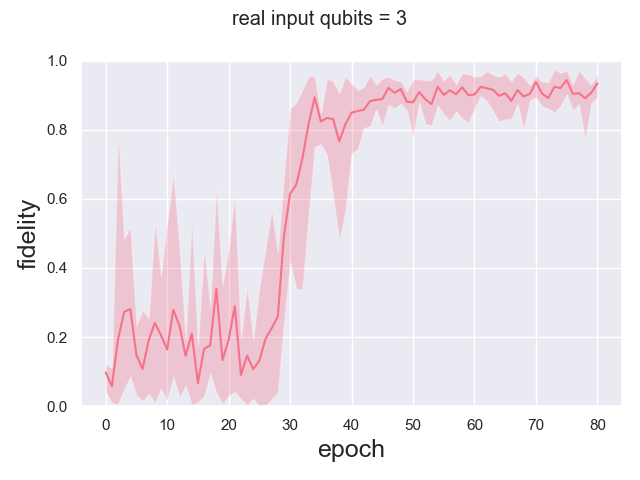
\includegraphics[width=0.3\linewidth]{figures/sqgans_size=3/fidelity.png}
  }
  \subfloat{
    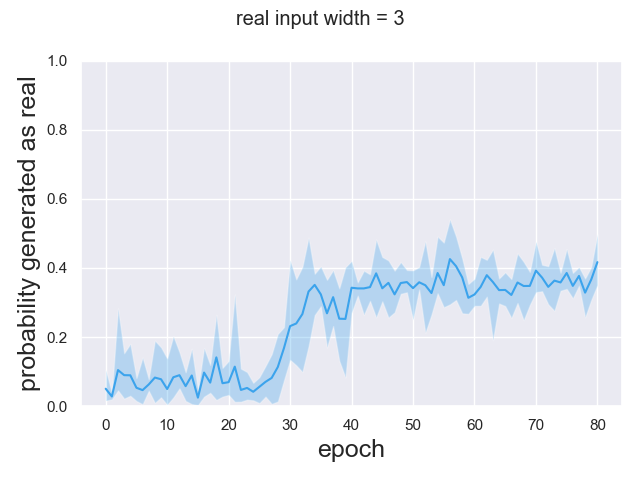
\includegraphics[width=0.3\linewidth]{figures/sqgans_size=3/probability_generated_as_real.png}
  }
  \subfloat{
    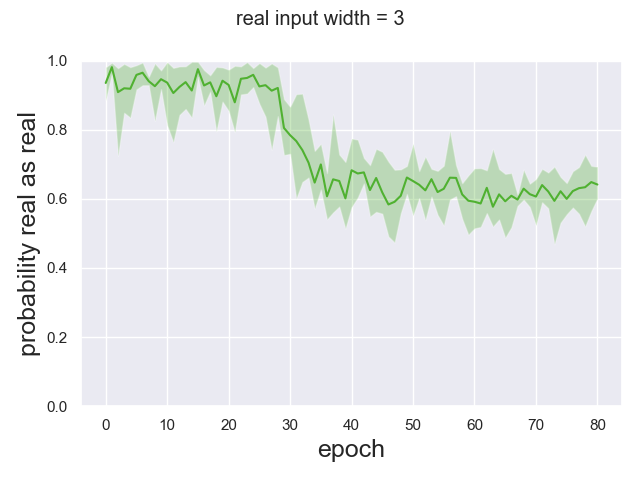
\includegraphics[width=0.3\linewidth]{figures/sqgans_size=3/probability_real_as_real.png}
  }


  \subfloat{
    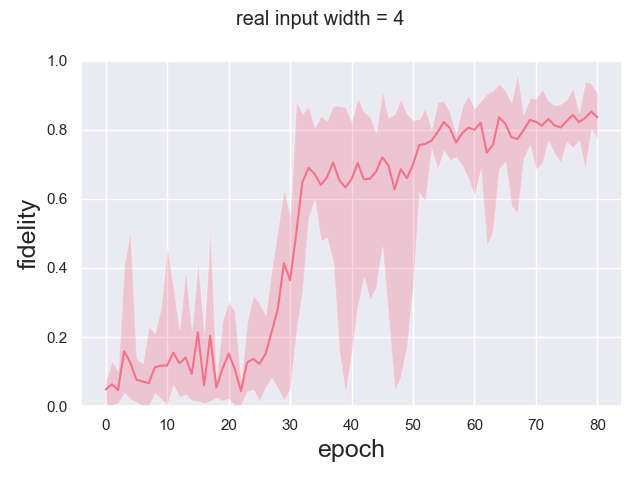
\includegraphics[width=0.3\linewidth]{figures/sqgans_size=4/fidelity.png}
  }
  \subfloat{
    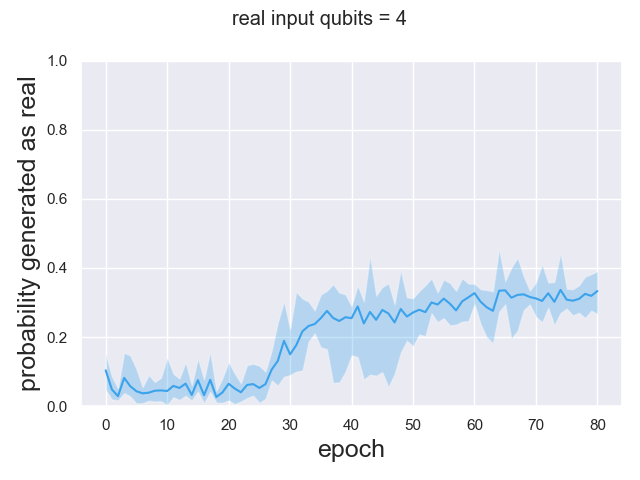
\includegraphics[width=0.3\linewidth]{figures/sqgans_size=4/probability_generated_as_real.png}
  }
  \subfloat{
    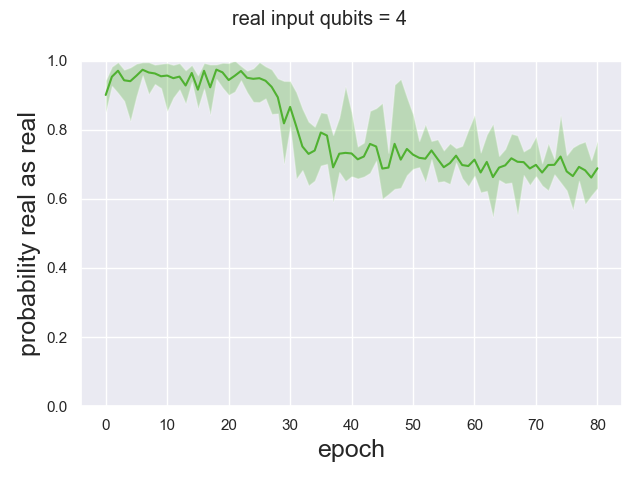
\includegraphics[width=0.3\linewidth]{figures/sqgans_size=4/probability_real_as_real.png}
  }

  \subfloat[Fidelity between real and \\generated state]{
    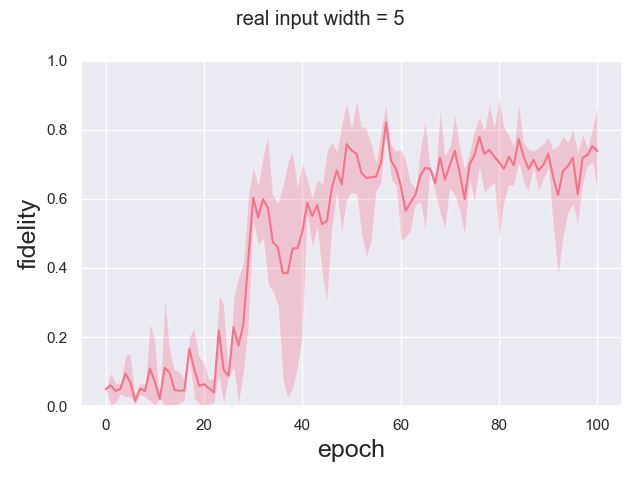
\includegraphics[width=0.3\linewidth]{figures/sqgans_size=5/fidelity.png}
  }
  \subfloat[Probability of classifying \\generated state as real]{
    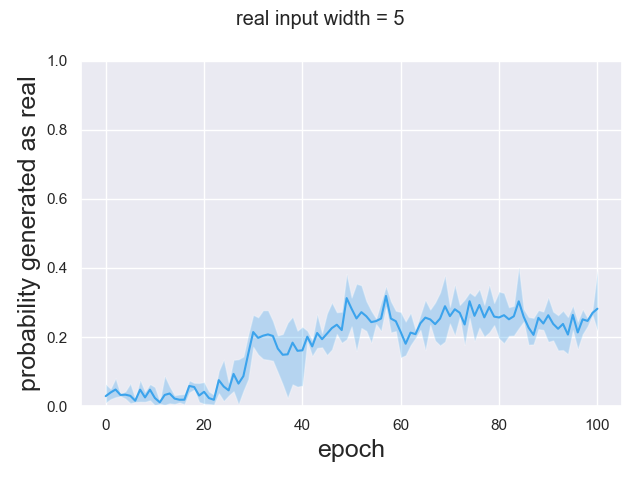
\includegraphics[width=0.3\linewidth]{figures/sqgans_size=5/probability_generated_as_real.png}
  }
  \subfloat[Probability of classifying real state as real]{
    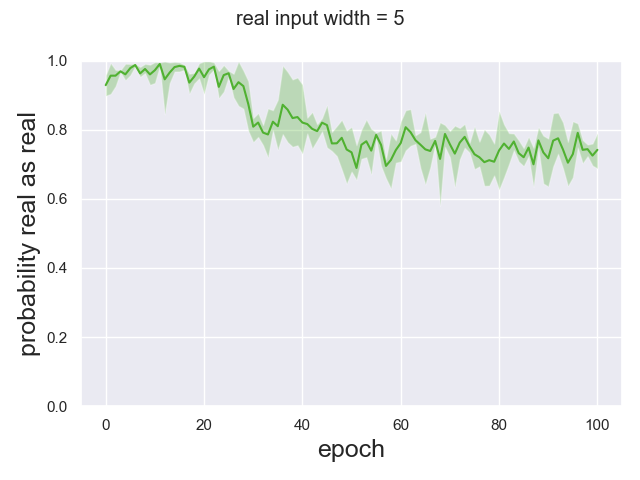
\includegraphics[width=0.3\linewidth]{figures/sqgans_size=5/probability_real_as_real.png}
  }
  \caption{The solid line represents the average value and the shaded area
    represents the range from 5 different experiments. The generator has the
    number of layers equal to the width of real input the discriminator has one
    more layer than the generator. In each epoch generator is optimized for 11 iterations and
  discriminator for 111. }
  \label{fig:sqgans_res_3}
\end{figure}
\subsubsection{Results For Mixed State Real Input}
If the real input source can provide more than one state, we can say that the
generator is learning mixed state of all the input states. Dallaire-Demers et
al. \cite{Dallaire_Demers_2018} trained a simple 2 qubits circuit with two real
input states $\ket{0}$ or $\ket{1}$. In this setup \textbf{Label} wires consist
of one qubit and also takes values $\ket{0}$ or $\ket{1}$, effectively learning
$CNOT$ gate. This strategy do not have generalize well in to more complex cases.
First, if there is more than one non-$\ket{0}$ input state, there would have to
be a separate $CNOT$ gate for each state. Second, the number of qubits necessary
for the \textbf{Label} wires grows logarithmically with the number of real input
states. Both of those cause the circuit to grow in width and depth.

Another approach we explored was to insert $R_x(\lambda_k)$ parametrized
rotation gates between each layer of the generator and discriminator. The
generator is essentially learning how to rotate input state $\ket{0}$ to some
desired real input state $\ket{r_k}$. Then, if for each $k$ the rotation is
pushed in different direction, the final generator might give different output
state for each $\lambda_k$. However, in our experiments the generator was always
learning to ignore the $R_x(\lambda_k)$ and in the end was only able to produce
one, slightly distorted, state independent of $\lambda_k$.

\subsection{Conclusions}
We have experimentally evaluated SQGANs and confirmed their ability to learn
pure quantum state. However, the problems with labeled states and small
circuit width for which the training succeeds prevented us from succeeding in
mixed state learning.

The very important aspect of generative models is ability to generate new,
unseen before, samples. In SQGANs this is theoretically possible by using the
textbf{Batch} register. However, it is not straight forward to use this register
in the intended way. First, the task of generating random quantum state is not
trivial on its own. Second, all the problems associated with the label state
$\lambda$ also apply to the random state $z$. 

Because of the above, we decided not to pursue the exploration of SQGANs further
and turned into other methods.


\section{Wasserstein Quantum GANs (WQGANs)}
  


%%% Local Variables:
%%% mode: latex
%%% TeX-master: "../main"
%%% End:
\chapter{Unseen Quantum State Generation}
\label{chapter:my_contribution}
In the previous chapter we evaluated two different types of quantum GANs. The
common problem of those is the inability to generate new, unseen states. In this
chapter we propose the hybrid classical-quantum framework that can overcome this limitation. 

Our idea is based WQGANs and how the quantum Wasserstein distance is
approximated during the training. The discriminator at every step approximates
the distance between some fixed, real input state and the generated state which
changes after each iteration. However, the discriminator never needs an access to
the actual real input state, it only operates on the set of measured
expectations. 

Given a parametrized circuits $U$
and set of parameters $\Theta = \{\theta_i\}$ and a set of operators $H =
\{H_j\}$, we prepare a set of vectors of expectations $S$. Each vector $s_{\theta_i}
\in S$ contains the expectations of the circuit $U(\theta_i)$, such that
$s_{\theta_i}^{(j)} = \langle H_j \rangle_{U(\theta_i)} $.

Assuming that all the vectors in $S$ come from the same distribution $p_S$,
the proposed framework is defined in two parts as follows:
\begin{enumerate}
\item \textit{Classical}: Takes as the input set $S$ and uses it to learn a function $f:
  \mathbb{R}^{n} \to \mathbb{R}^{|H|}$. Given an arbitrary vector $g \in
  \mathbb{R}^n$ (e.g. random noise), this function produces a new vector $s' =
  f(g)$ such that $s' \sim p_S$.  
\item \textit{Quantum}: Takes $s'$ as the input and uses it as
  expectations of real input source in the WQGANs setting described in the
  previous chapter. The generator trained using $s'$ produces new, unseen before
  quantum state. The WQGANs optimization objective from Equation
  \ref{eq:wqgans_optimization_objective} becomes:
  \begin{equation}
    \max_{w}{\min_{\theta}{\mathcal{L}(w, \theta)}} = \max_{w}{\min_{\theta}{(\sum_{i=1}^Nw_i(s^{\prime(i)} - Tr[G(\theta)H_i]))}} 
    \label{eq:wqgans_optimization_objective_unseen}
  \end{equation}
\end{enumerate}

Once the function $f$ is learnt, it can be used arbitrary many times to produce
new vectors of expectations.
With those vectors, it is possible to generate new quantum states that come from
some circuit $U(\theta')$, without ever knowing $U$ or $\theta'$.
In the following sections, we show how exactly the function $f$ can be obtained
for two different cases. 
\section{Labeled State Generation}
If the quantum state produced by the circuit $U$ can be labeled by some continuous
variable, we can use this variable to find the function $f$.

Specifically, here we assume that each parameter $\theta_i^{(j)}$ is described by some
function, i.e. $\theta_i = \theta(g_i) = [\theta^{(1)}(g_i), \theta^{(2)}(g_i), \ldots,
\theta^{(l)}(g_i)]$, for some $g_i \in V \subseteq 
\mathbb{R}$, where $l$ is the number of parameters in the circuit $U$.
We also assume that the expectations of the state produced by the
circuit $U(\theta(g_i))$, can be described by some other functions,
i.e. $s_{\theta_i} = s(g_i) = [s^{(1)}(g_i), s^{(2)}(g_i), \ldots,
s^{(|H|)}(g_i)]$, $s^{(j)}: V \to [-1; 1]\ \forall_{j \in 1,\ldots,|H|}$.
Then, the input to the classical part of the framework is the set $S$, together with
corresponding $g_i$ for each $s_{\theta_i} = s(g_i) \in S$.
To find $s^{(j)}\ \forall_{j=1,\ldots,|H|}$ functions interpolation is
sufficient. So, the function $f: V \to \mathbb{R}^{|H|}$ simply takes
any value of $g \in V$ and returns the expectations for this value using
interpolations of functions $s^{(j)}$.

\subsection{Evaluation Results}
This approach can be used when $U$ is the topological phase transition circuit from
Appendix \ref{apx:topological_phase_transition_ansatz}. All the parameters of
this circuit can be described by three functions $\theta_v, \theta_w, \theta_r$
over $V = [-1; 1]$. To prepare the input to the classical part 
 $m$ ($m = |S|$) values of $g \in V$ are sampled and the expectations of $U(\theta_v(g_i),
\theta_w(g_i), \theta_r(g_i))\ \forall_{i=1,\ldots,m}$ are calculated for all operators $H_i
\in H$. Similarly as in the WQGANs chapter, $H$ is chosen to be a
set of all k-length Pauli Strings.
This data is used to interpolate the expectation functions for those operators.  

In Figure \ref{fig:phase_exps} interpolated expectations of the circuit for
$k=3$ and $m=11$ are plotted (only subset of the expectation is plotted for readability).

\begin{figure}[htbp!]
  \captionsetup[subfigure]{labelformat=empty}
  \centering
  \subfloat{
    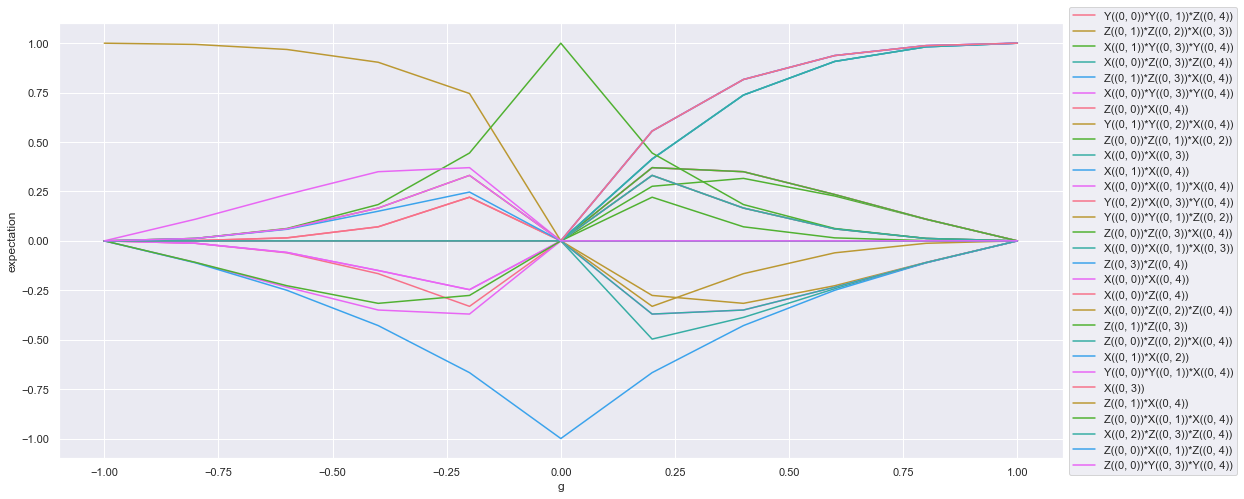
\includegraphics[width=1\linewidth]{figures/phase_exps/plot.png}
  }
  \caption{Interpolated expectations of topological phase transition circuit (Appendix
    \ref{apx:topological_phase_transition_ansatz}) with 5 qubits width for $10$
    random 3-Pauli Strings operators. Interpolation using evenly
    spaced 11 values of the parameter $g \in [-1; 1]$. 
  }
  \label{fig:phase_exps}
\end{figure}

The interpolated expectations are used to learn the quantum states for
the values of $g$ that were not part of the classical input. In Figure
\ref{fig:wqgans_res_interpolated_1} we see fidelity and Wasserstein distance
between the real input states and the ones learnt using the interpolated
expectations.
Those results are comparable with the ones obtained by learning from known
expectations (Figure \ref{fig:wqgans_res_1}).

\begin{figure}[htbp!]
  \captionsetup[subfigure]{labelformat=empty}
  \centering
  \subfloat{
    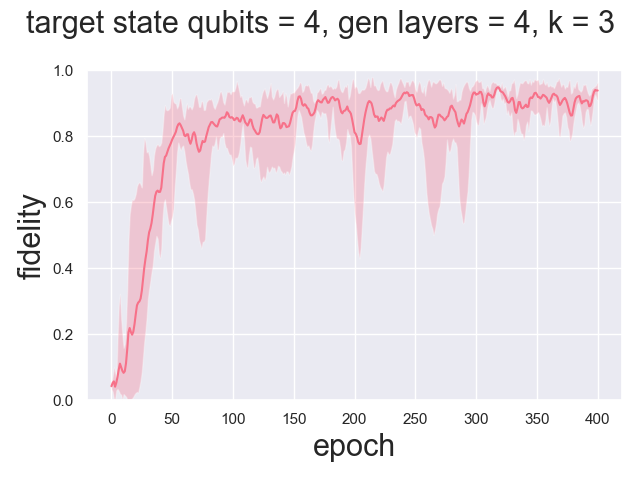
\includegraphics[width=0.25\linewidth]{figures/wqgans_phase_size=4_k=3_gen=4_interpolation/fidelity.png}
  }
  \subfloat{
    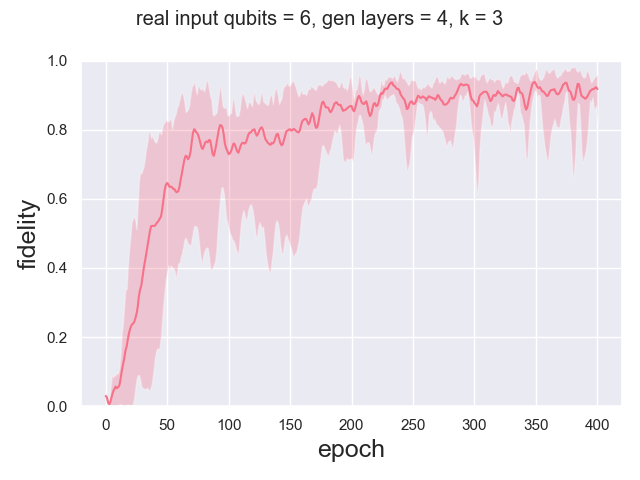
\includegraphics[width=0.25\linewidth]{figures/wqgans_phase_size=6_k=3_gen=4_interpolation/fidelity.png}
  }
  \subfloat{
    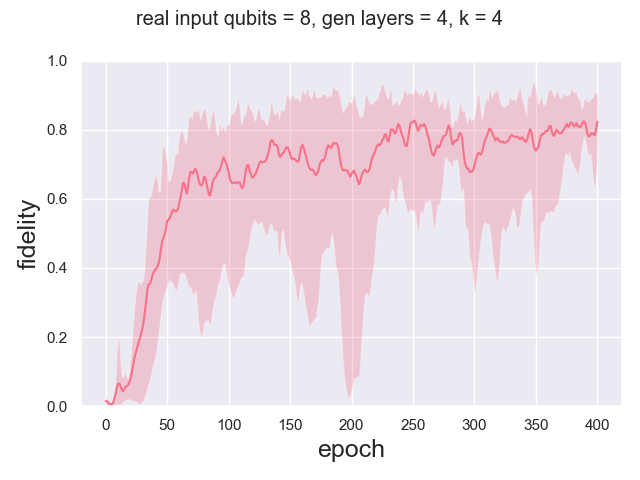
\includegraphics[width=0.25\linewidth]{figures/wqgans_phase_size=8_k=4_gen=4_interpolation/fidelity.png}
  }
  \subfloat{
    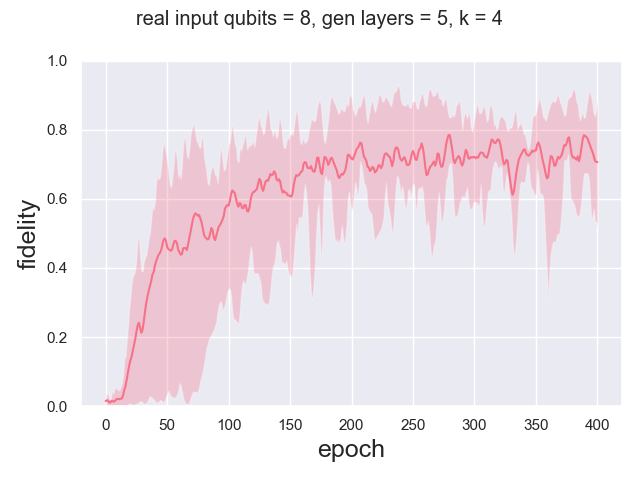
\includegraphics[width=0.25\linewidth]{figures/wqgans_phase_size=8_k=4_gen=5_interpolation/fidelity.png}
  }

  \subfloat{
    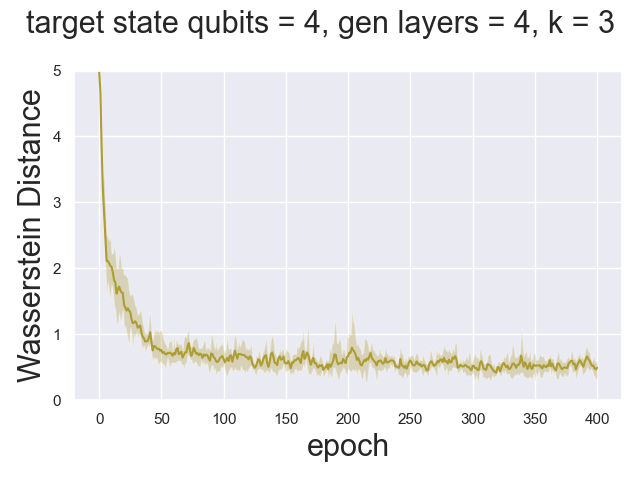
\includegraphics[width=0.25\linewidth]{figures/wqgans_phase_size=4_k=3_gen=4_interpolation/Wasserstein_Distance.png}
  }
  \subfloat{
    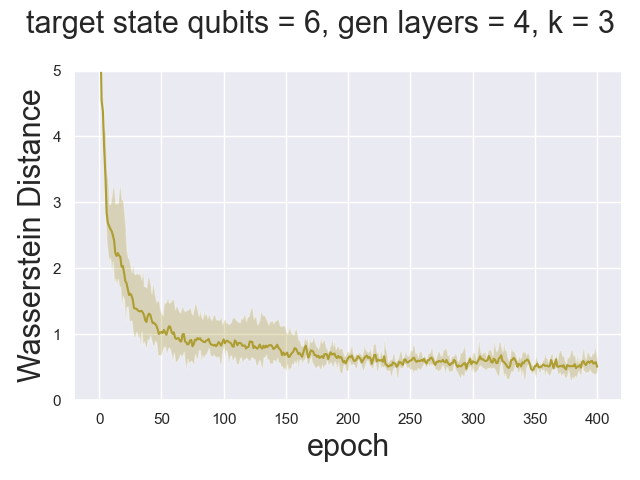
\includegraphics[width=0.25\linewidth]{figures/wqgans_phase_size=6_k=3_gen=4_interpolation/Wasserstein_Distance.png}
  }
  \subfloat{
    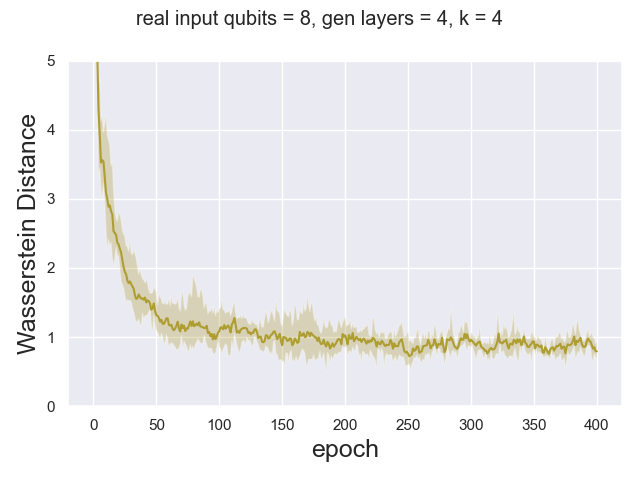
\includegraphics[width=0.25\linewidth]{figures/wqgans_phase_size=8_k=4_gen=4_interpolation/Wasserstein_Distance.png}
  }
  \subfloat{
    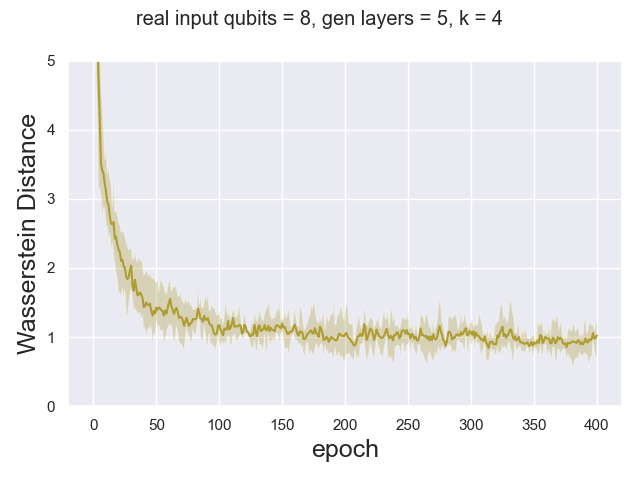
\includegraphics[width=0.25\linewidth]{figures/wqgans_phase_size=8_k=4_gen=5_interpolation/Wasserstein_Distance.png}
  }
  \caption{Results for topological phase transition circuit (ansatz Appendix
    \ref{apx:topological_phase_transition_ansatz}) using interpolated expectations.
    The solid line represents the average value and the shaded area
    represents the range from 5 different experiments. The upper row shows the
    fidelity and the bottom row shows the corresponding Wasserstein distance. In all the
    experiments the generator is built using ansatz from Appendix
    \ref{apx:sqgans_ansatz}. }
  \label{fig:wqgans_res_interpolated_1}
\end{figure}

\subsubsection{String Order Parameters}

In their work Smith et. al\cite{smith2020crossing} define two
string order parameters
\begin{equation}
\begin{split}
S^\mathbb{1} =  & \bra{\psi}(\prod_{i=3}^{N-2}X_i)\ket{\psi} \\
S^{ZY} =  & \bra{\psi}Z_2Y_3(\prod_{i=4}^{N-3}X_i)Y_{N-2}Z_{N-1}\ket{\psi},
\end{split}
\end{equation}
where $N$ is the width of the circuit and $\ket{\psi}$ is the final state
obtained by the topological phase transition circuit from Appendix
\ref{apx:topological_phase_transition_ansatz}.
The measurements of $S^{\mathbb{1}}$ and $S^{ZY}$ on states learnt using the
interpolated expectations are shown in Figure \ref{fig:string_order_1}. The
obtained results closely follow the expected value and the phase transition
point at $g=0$ is clearly distinguishable.

\begin{figure}[htbp!]
  \captionsetup[subfigure]{labelformat=empty}
  \centering
  \subfloat{
    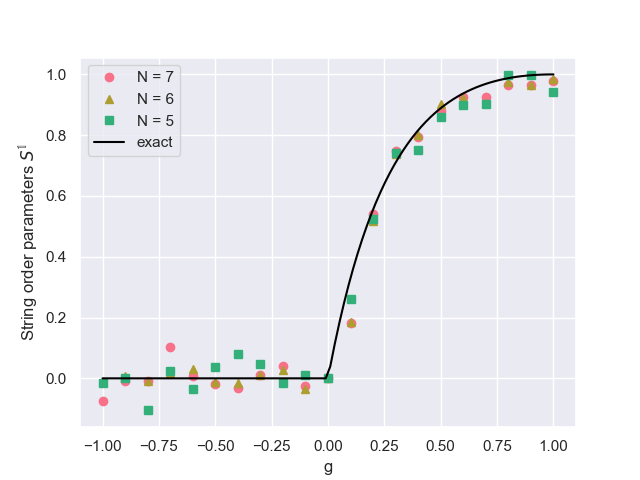
\includegraphics[width=0.5\linewidth]{figures/string_order_s1/plot.png}
  }
  \subfloat{
    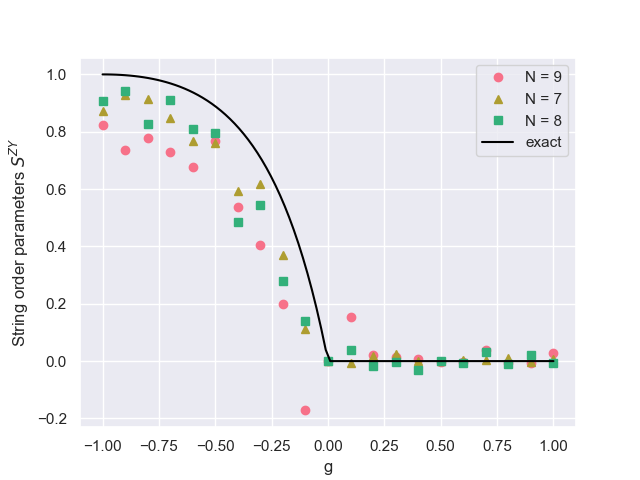
\includegraphics[width=0.5\linewidth]{figures/string_order_szy/plot.png}
  }
  \caption{String order parameters $S^\mathbb{1}$ and $S^{ZY}$ measured on the
    generic generator from Appendix \ref{apx:sqgans_ansatz}, trained using the
    interpolated expectations, for different width of circuit $N$.
    The phase transition at $g=0$ is clearly visible,
    the results are very close to the exact ones.}
\label{fig:string_order_1}
\end{figure}

\subsection{Conclusions}
Using the interpolated expectations allows to learn unknown quantum states.
In all the experiments generic generator ansatz was used, meaning that also the
design of $U$ and its parametrization was unknown to the quantum Generator and
Discriminator.

Although the setup described here assumes one dimensional variable $g$, this
notion can be extended to multi-variable case where $g \in V \subseteq
\mathbb{R}^m$.



\section{Unlabeled State Generation}
In the general case the assumptions from the previous Section do not hold and
more powerful tools are need to find the function $f$. However, following the assumption
that all vectors in input set $S$ come from the same distribution $p_S$, we can use
the generative modeling to learn the function $f$. In particular, here we use
classical Wasserstein Generative Adversarial Networks (WGANs) to approximate the
distribution $p_S$ and later use the classical Generator as the function $f$ to
produce the vectors $s'$. 

\subsection{Evaluation Results}
We use this technique to generate new, previously unseen states from butterfly circuit
(Appendix \ref{apx:butterfly_ansatz}). First, we generate the set $S$ and use it
to train a simple WGAN-GP \cite{gulrajani2017improved}, with penalty factor
$10$. We use simple 2-layers deep neural network (DNN), with input dimension $16$ and
layer dimensions $64$ and $128$, for both, generator and
discriminator. We use Adam optimizer \cite{kingma2017adam} with the following
parameters $\beta_1 = 0.9$, $\beta_2 = 0.999$, $\hat{\epsilon} = 1e - 7$ and
learning rate of $0.001$. 

For the states generated in this way, it is not possible to calculate the fidelity, so we
relay on Wasserstein distance to evaluate the results. As shown in the previous
chapter, the decrease in Wasserstein distance is strongly correlated with
the increase in fidelity. In Figure \ref{fig:wqgans_res_gans_1} results for
several different sizes of real input are presented. We use generator with the
same architecture as the real input source, to see whether the expectations
generated by classical GANs could be measured from the real input circuit.
Wasserstein distance very quickly drops below $1$, which should correspond to
fidelity of more than $0.8$ based on the previous observations. However, it
always plateaus before dropping to 0, which indicated that the classical
generator does not produce expectations exactly from the $p_S$ distribution.

\begin{figure}[htbp!]
  \captionsetup[subfigure]{labelformat=empty}
  \centering
  \subfloat{
    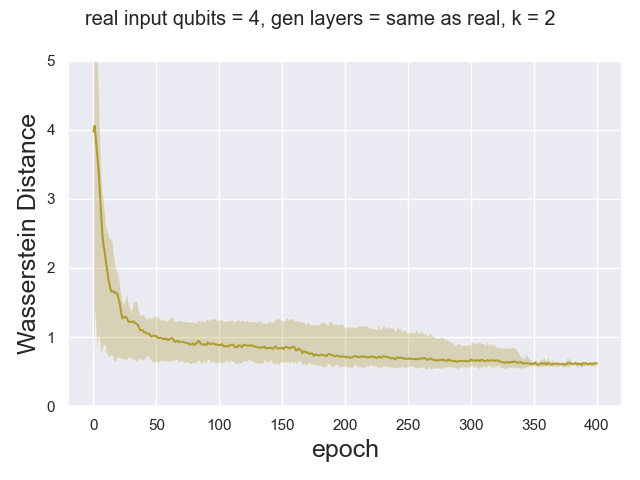
\includegraphics[width=0.33\linewidth]{figures/wqgans_butterfly_size=4_k=2_gen=same_as_real_gan/Wasserstein_Distance.png}
  }
  \subfloat{
    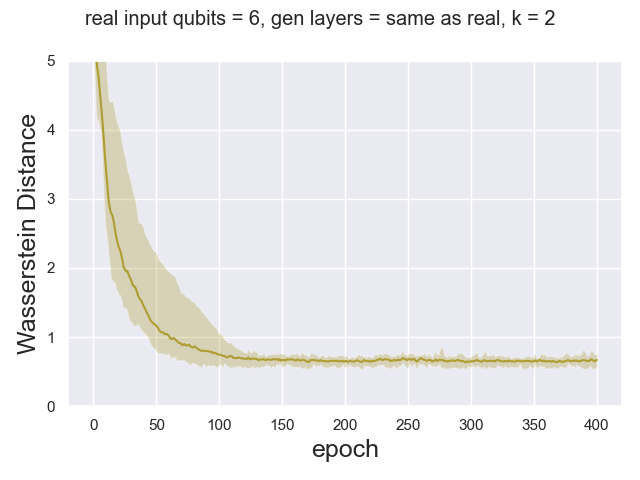
\includegraphics[width=0.33\linewidth]{figures/wqgans_butterfly_size=6_k=2_gen=same_as_real_gan/Wasserstein_Distance.png}
  }
  \subfloat{
    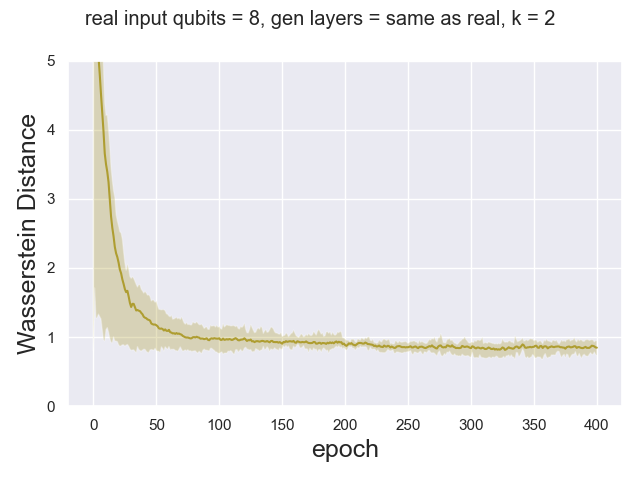
\includegraphics[width=0.33\linewidth]{figures/wqgans_butterfly_size=8_k=2_gen=same_as_real_gan/Wasserstein_Distance.png}
  }
  \caption{Wasserstein Distance for butterfly circuit (ansatz Appendix
    \ref{apx:butterfly_ansatz}) using expectations generated with GANs. Results
    for training set size $|S| = 256$ for $k=4,6$ and $|S| = 512$ for $k=8$. 
    The solid line represents the average value and the shaded area
    represents the range from 5 different experiments. In all the
    experiments the generator is built using the same butterfly circuit.
    \ref{apx:sqgans_ansatz}. }
  \label{fig:wqgans_res_gans_1}
\end{figure}

\subsection{Conclusions}
We have demonstrated the ability to generate unseen quantum state, with the
expectations generated by classical GANs. Despite using basic and shallow DNN
for the classical generator and discriminator, the generated expectations were
very close to the ones measured from the generated quantum state as indicated by
measured Wasserstein distance. Using more sophisticated or deeper architecture
for classical GANs could yield better results or decrease the required training
size and is an interesting direction for the further research. 

%%% Local Variables:
%%% mode: latex
%%% TeX-master: "../main"
%%% End:
\chapter{Results}\label{chapter:results}
\chapter{Conclusions}\label{chapter:conclusions}
The field of quantum machine learning is currently in an early, exploratory
stage. There have been many attempts to bring the successful classical machine
learning ideas into the quantum realm. In this work we took a closer look at
Generative Adversarial Networks and their realization on the quantum machines.
We evaluated two types of quantum GANs, SQGANs\cite{Dallaire_Demers_2018} and
WQGANs\cite{depalma2020quantum}, using pure and mixed real input sources of
different sizes and circuit designs. Both of those networks are able to learn to
generate previously seen quantum states for small real input sources.
However, according to our evaluation, WQGANs are more robust, easier to train
and work for wider inputs. We also confirmed, that the quantum
Wasserstein distance approximated by WQGANs is closely correlated with fidelity
and is a good metric to measure the similarity of quantum states.

Finally, by using the insights from the above evaluation, we proposed a new way
to generate unseen quantum states. We combined the classical generative modeling 
with WQGANs to train parametrized quantum circuit able to generate new quantum
states. We showed experimentally, that the quantum states generated by our
method follow the distribution of the states used to train the generative networks.

All the attempts so far, including this work, concentrated on small input of
several or maximum dozen qubits. An important are to explore is the
scalability of quantum GANs for wider inputs, especially on the currently available NISQ machines.  
Another interesting question is, how could the unseen states be generated
in the fully quantum manner, without the need to use the classical computer. 

%%% Local Variables:
%%% mode: latex
%%% TeX-master: "../main"
%%% End:
\appendix{}

% TODO: appendix chapter
\chapter{SGANs approximates Jensen–Shannon Divergence}
\label{apx:JSD}
Kullback-Leibler (KL) divergence, by definition is stated as follows
\begin{equation*}
  D_{KL}(p || q) = \int_xp(x)log(\frac{p(x)}{q(x)})dx. 
\end{equation*}

Jensen-Shannon (JS) divergence is defined using KL divergence is stated as follows
way
\begin{equation*}
D_{JS}(p || q) = \frac{1}{2}(D_{KL}(p || \frac{p+q}{2}) + D_{KL}(q || \frac{p+q}{2})).
\end{equation*}


The SGANs loss function, using continuous expectation definition, is stated as follows
\begin{equation*}
  \begin{split}
    \mathcal{L}(G, D) & =  \mathbb{E}_{x \sim p_r(x)}[\log{D(x)}] +  \mathbb{E}_{x \sim p_g(x)}[\log{1 - D(x)}] \\
    & = \int_x(p_r(x)\log{(D(x))} + p_g(x)\log{(1-D(x))})dx \\
    & = \int_xf(x)dx.
  \end{split}
\end{equation*}

First, to find the optimal discriminator $D^*$, we find the maximum of the
function $f(x)$.

\begin{equation*}
\begin{split}
  \frac{df(x)}{dx} & = \frac{p_r(x)}{\ln{10} * D^*(x)} - \frac{p_g(x)}{\ln{10} * (1-D^*(x))} = 0 \Rightarrow \\
  D^*(x) & = \frac{p_r(x)}{p_r(x) + p_g(x)}
\end{split}
\end{equation*}
So the loss function for $D^*(x)$ takes the form
\begin{equation}
  \mathcal{L}(G, D^*) = \int_x(p_r(x)\log{(\frac{p_r(x)}{p_r(x) + p_g(x)})} + p_g(x)\log{(\frac{p_g(x)}{p_r(x) + p_g(x)})}dx.
  \label{eq:sgan_optimal_disc}
\end{equation}
For the optimal generator $G*$, the probabilities of predicting generated and
real data are equal, i.e. $p_r=p_g$, and the loss function becomes constant
\begin{equation}
\mathcal{L}(G^*, D^*) = -log{4}.
\label{eq:sgan_optimal_gen_disc}
\end{equation}
Now, we can rewrite Equation \ref{eq:sgan_optimal_disc} using the definition of KL
divergence
\begin{equation*}
  \begin{split}
    \mathcal{L}(G, D^*) & = D_{KL}(p_r || p_r + p_g) + D_{KL}(p_g || p_r + p_g) \\ 
    & = D_{KL}(p_r || \frac{p_r + p_g}{2}) - \log{2} + D_{KL}(p_g || \frac{p_r + p_g}{2}) -\log{2} \\
    & = D_{JS}(p_r || p_g) - log{4}
  \end{split}
\end{equation*}
Using the Equation \ref{eq:sgan_optimal_gen_disc} for optimal loss we see that
\begin{equation*}
  \mathcal{L}(G^*, D^*) = D_{JS}(p_r || p_g) -log{4} =  - log{4}
\end{equation*}
from which we conclude that for optimal case of training the Jensen-Shannon
divergence is $0$ and the distributions $p_r$ and $p_q$ are equal. $\qed$

% If there are several additions you want to add, but they do not fit into the thesis itself, they belong here.

% \section{Detailed Addition}

% Even sections are possible, but usually only used for several elements in, e.g.\ tables, images, etc.
\let\oldclearpage\clearpage
\let\clearpage\relax
\chapter{Circuits}
\section{Generic Ansatz}
\label{apx:sqgans_ansatz}
\begin{figure}[htbp!]
  \begin{tikzcd}
    \qw &  \gate{R_x(\theta_{(x,1)}^{(i)})} & \gate{R_z(\theta_{(z,1)}^{(i)})} &
    \gate[2, disable auto height]{R_{zz}(\theta_{(1,2)}^{(i)})} & \qw & \qw \\
    \qw &  \gate{R_x(\theta_{(x,2)}^{(i)})} & \gate{R_z(\theta_{(z,2)}^{(i)})} &
    \qw & \gate[2, disable auto height]{R_{zz}(\theta_{(2,3)}^{(i)})} & \qw \\
    \qw &  \gate{R_x(\theta_{(x,3)}^{(i)})} & \gate{R_z(\theta_{(z,3)}^{(i)})} &
    \gate[2, disable auto height]{R_{zz}(\theta_{(3,4)}^{(i)})} & \qw  & \qw \\ 
    \qw &  \gate{R_x(\theta_{(x,4)}^{(i)})} & \gate{R_z(\theta_{(z,4)}^{(i)})} &
    \qw & \vdots \\
     & \vdots & \vdots & \vdots & \vdots & \\
    \qw &  \gate{R_x(\theta_{(x,w-2)}^{(i)})} & \gate{R_z(\theta_{(z,w-2)}^{(i)})} &
    \gate[2, disable auto height]{R_{zz}(\theta_{(w-2,w-1)}^{(i)})} & \vdots \\ 
    \qw &  \gate{R_x(\theta_{(x,w-1)}^{(i)})} & \gate{R_z(\theta_{(z,w-2)}^{(i)})} &
    \vdots & \gate[2, disable auto height]{R_{zz}(\theta_{(w-1,w)}^{(i)})} & \qw \\
    \qw & \gate{R_x(\theta_{(x,w)}^{(i)})} & \gate{R_z(\theta_{(z,w)}^{(i)})} &
    \qw & \qw  & \qw
  \end{tikzcd}
  \caption{Single layer of the generic ansatz used for generator and
    discriminator circuits \cite{Dallaire_Demers_2018}. Circuit parametrized by
    vector $\theta$, where $i$ denotes the layer number and $w$ denotes the
    width of the circuit.
  }
  \label{fig:phase_circuit_apx}
\end{figure}
\section{Topological Phase Transition Ansatz}
This circuit was used by Smith et al. \cite{smith2020crossing} to study
transitions between different states of matter. It is essentially a matrix
product state (MPS) stated in the quantum circuit form.
\label{apx:topological_phase_transition_ansatz}
\begin{figure}[htbp!]
  \begin{tikzcd}
    \lstick{$\ket{0}$} & \gate[2, disable auto height]{U_1(g)} & \qw & \qw & \qw &
    \qw & \qw & \qw \\
    \lstick{$\ket{0}$} & & \gate[2, disable auto height]{U(g)}  & \qw & \qw & \qw & \qw & \qw \\
    \lstick{$\ket{0}$} & \qw & \qw & \gate[2, disable auto height]{U(g)}  & \qw & \qw & \qw & \qw \\
    \lstick{$\ket{0}$} & \qw & \qw & \qw & \qw & \ldots  \\
    \vdots & & & & &\ldots & \gate[2, disable auto height]{U(g)} & \qw \\
    \lstick{$\ket{0}$} & \qw & \qw & \qw & \qw & \qw & \qw & \qw \\
  \end{tikzcd}
  \caption{The topological phase transition circuit studied in \cite{smith2020crossing} }
  \label{fig:phase_circuit_apx}
\end{figure}
\begin{figure}[htbp!]
  \begin{tikzcd}
    \lstick{$\ket{0}$} & \gate{H} & \ctrl{1} & \qw & \qw & \gategroup[2, steps=3,
    style={dashed, fill=blue!20, inner xsep=2pt}, background]{{
        Only for g > 0}}\qw & \ctrl{1} & \qw & \qw \\
    \lstick{$\ket{0}$} & \qw & \targ{} & \gate{Z} & \gate{R_y(\theta_r(g))} & \gate{H} & \targ{} &
    \gate{H} & \qw
  \end{tikzcd}
  \caption{The schema of $U_1$ gate from the circuit in Figure \ref{fig:phase_circuit_apx}}
  \label{fig:phase_circuit_u1}
\end{figure}
\begin{figure}[htbp!]
  \begin{tikzcd}
    \lstick{$\ket{\cdot}$} & \gate{X} & \ctrl{1} & \gate{X} & \qw & \qw & \qw & \ctrl{1} &
     \qw & \gate{X} & \qw & \qw \\
     \lstick{$\ket{0}$} &  \gate{R_y(\theta_w(g))}  & \targ{} &  \gate{X} & \gate{R_y(\theta_w(g))} & \gate{X} &  \gate{R_y(\theta_v(g))}
     & \targ{} & \gate{X} & \gate{R_y(\theta_v(g))} & \gate{X} & \qw
  \end{tikzcd}
  \caption{The schema of $U$ gate from the circuit in Figure \ref{fig:phase_circuit_apx}}
  \label{fig:phase_circuit_u}
\end{figure}

Where
\begin{equation*}
  \begin{split}
    R_y(\theta) & = \begin{pmatrix}
      \cos{\frac{\theta}{2}} & -\sin{\frac{\theta}{2}} \\
      \sin{\frac{\theta}{2}} & \cos{\frac{\theta}{2}} 
    \end{pmatrix}, \\
    \theta_w(g) & = \arccos{\frac{sign(g)\sqrt{|g|}}{\sqrt{1+|g|}}},\ \theta_w \in [0, \pi], \\
    \theta_v(g) & = \arcsin{\frac{\sqrt{|g|}}{\sqrt{1+|g|}}},\ \theta_v \in [-\frac{\pi}{2}, \frac{\pi}{2}], \\
    \theta_r(g) & = 2\arcsin{\frac{1}{\sqrt{1+|g|}}},\ \theta_r \in [-\pi, \pi].
  \end{split}
\end{equation*}

\section{Butterfly Ansatz}
\label{apx:butterfly_ansatz}
\begin{figure}[htbp!]
\begin{tikzcd}
\lstick{$\ket{0}$} & \gate{R_x(\theta_{(1,1)})} & \ctrl{1} &
\gate{R_x(\theta_{(3,1)})} & \ctrl{2} & \qw & \gate{R_x(\theta_{(5,1)})} & \qw &
\ldots & \rstick[wires=9]{$\ket{\psi}$}\\
\lstick{$\ket{0}$} & \gate{R_x(\theta_{(1,2)})} & \gate{R_x(\theta_{(2,1)})}  &
\gate{R_x(\theta_{(3,2)})} & \qw & \ctrl{2} & \gate{R_x(\theta_{(5,2)})} & \qw &
\ldots & \\ 
\lstick{$\ket{0}$} & \gate{R_x(\theta_{(1,3)})} & \ctrl{1} &
\gate{R_x(\theta_{(3,3)})} & \gate{R_x(\theta{(4,1)})} & \qw & \gate{R_x(\theta_{(5,3)})} & \qw &
\ldots & \\
\lstick{$\ket{0}$} & \gate{R_x(\theta_{(1,4)})} & \gate{R_x(\theta_{(2,2)})}  &
\gate{R_x(\theta_{(3,4)})} & \qw & \gate{R_x(\theta{(4,2)})} & \gate{R_x(\theta_{(5,4)})} & \qw &
\ldots & \\ 
\lstick{$\ket{0}$} & \gate{R_x(\theta_{(1,5)})} & \ctrl{1} &
\gate{R_x(\theta_{(3,5)})} & \ctrl{2} & \qw & \gate{R_x(\theta_{(5,5)})} & \qw &
\ldots & \\ 
\lstick{$\ket{0}$} & \gate{R_x(\theta_{(1,6)})} & \gate{R_x(\theta_{(2,3)})}  &
\gate{R_x(\theta_{(3,6)})} & \qw & \ctrl{2} & \gate{R_x(\theta_{(5,6)})} & \qw &
\ldots & \\ 
\lstick{$\ket{0}$} & \gate{R_x(\theta_{(1,7)})} & \ctrl{1} &
\gate{R_x(\theta_{(3,7)})} & \gate{R_x(\theta{(4,3)})} & \qw & \gate{R_x(\theta_{(5,7)})} & \qw &
\ldots & \\ 
\lstick{$\ket{0}$} & \gate{R_x(\theta_{(1,8)})} & \gate{R_x(\theta_{(2,4)})}  &
\gate{R_x(\theta_{(3,8)})} & \qw & \gate{R_x(\theta{(4,4)})} & \gate{R_x(\theta_{(5,8)})} & \qw &
\ldots & \\
\lstick{$\ket{0}$} & \gate{R_x(\theta_{(1,9)})} & \qw  &
\gate{R_x(\theta_{(3,9)})} & \qw & \qw & \gate{R_x(\theta_{(5,9)})} & \qw &
\ldots & \\
\end{tikzcd}
\caption{The butterfly circuit for 9 qubits. For each $j$-th power of $2$ that the
  width of the circuit exceeds, the next layer is added that consist of $R_x$
  gates on each qubit and controlled $R_x$ gate between $i$-th and $i+2^j$-th qubits (continued below).}
\end{figure}
\begin{figure}[htbp!] \ContinuedFloat
\begin{tikzcd}
  \lstick[wires=9]{$\psi$} & \ldots & \ctrl{4} & \qw & \qw &
  \qw & \gate{R_x(\theta_{(7,1)})} & \ctrl{8} & \qw \\
  & \ldots & \qw & \ctrl{4} & \qw & \qw  &
  \gate{R_x(\theta_{(7,2)})} & \qw & \qw\\
  & \ldots & \qw & \qw & \ctrl{4} & \qw &
  \gate{R_x(\theta_{(7,3)})}  \qw & \qw & \qw\\
  & \ldots & \qw & \qw & \qw & \ctrl{4}  &
  \gate{R_x(\theta_{(7,4)})}  \qw & \qw & \qw\\
  &  \ldots &\gate{R_x(\theta_{(6,1)})} & \qw & \qw & \qw &
  \gate{R_x(\theta_{(7,5)})}  \qw & \qw & \qw\\
  & \ldots & \qw & \gate{R_x(\theta_{(6,2)})}  & \qw & \qw &
  \gate{R_x(\theta_{(7,6)})}  \qw & \qw & \qw\\
  & \ldots & \qw & \qw & \gate{R_x(\theta_{(6,3)})} & \qw &
  \gate{R_x(\theta_{(7,7)})}  \qw & \qw & \qw\\ 
  &  \ldots &\qw & \qw & \qw & \gate{R_x(\theta_{(6,4)})}  &
  \gate{R_x(\theta_{(7,8)})}  \qw & \qw & \qw\\
  & \ldots & \qw & \qw & \qw & \qw &
  \gate{R_x(\theta_{(7,9)})}  & \gate{R_x(\theta_{(8,1)})} & \qw \\
\end{tikzcd}
\caption{The butterfly circuit for 9 qubits. For each $j$-th power of $2$ that the
    width of the circuit exceeds, the next layer is added that consist of $R_x$
    gates on each qubit and controlled $R_x$ gate between $i$-th and $i+2^j$-th qubits }
\end{figure}
\chapter{WQGANs Additional Results}
\label{apx:wqgans_pahse_results}
\begin{figure}[htbp!]
  \captionsetup[subfigure]{labelformat=empty}
  \centering
  \subfloat{
    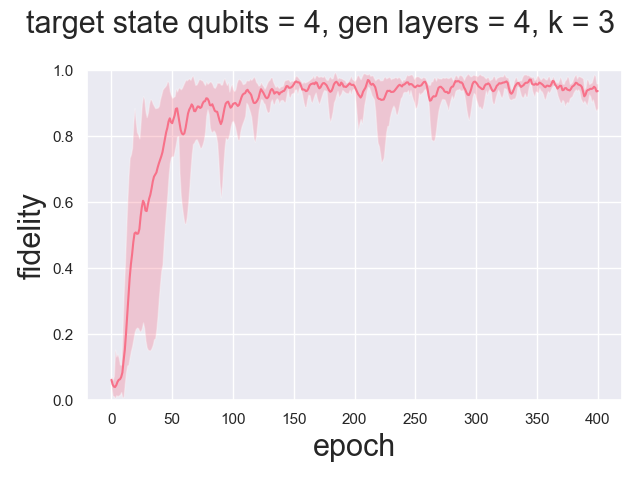
\includegraphics[width=0.3\linewidth]{figures/wqgans_phase_size=4_k=3_gen=4/fidelity.png}
  }
  \subfloat{
    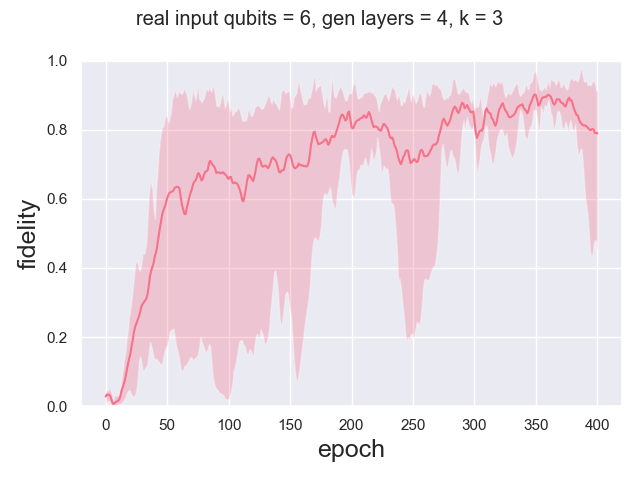
\includegraphics[width=0.3\linewidth]{figures/wqgans_phase_size=6_k=3_gen=4/fidelity.png}
  }
  \subfloat{
    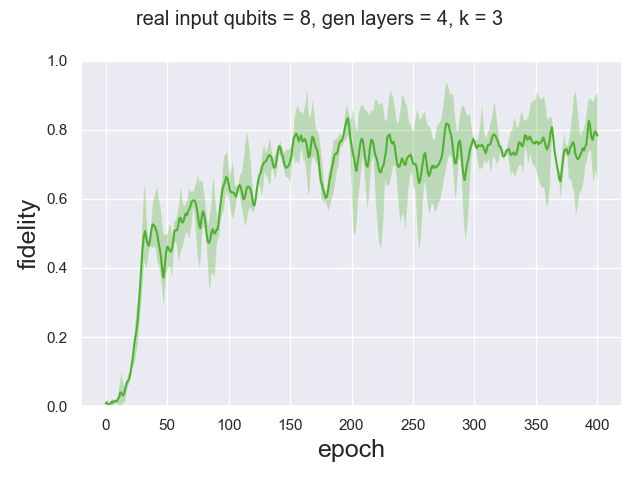
\includegraphics[width=0.3\linewidth]{figures/wqgans_phase_size=8_k=3_gen=4/fidelity.png}
  }

  \subfloat{
    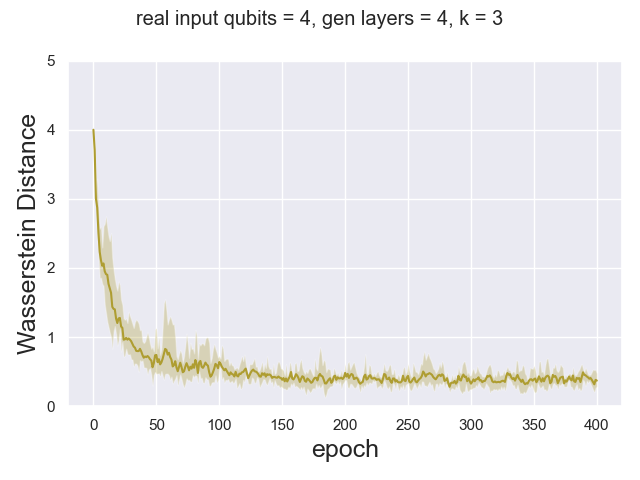
\includegraphics[width=0.3\linewidth]{figures/wqgans_phase_size=4_k=3_gen=4/Wasserstein_Distance.png}
  }
  \subfloat{
    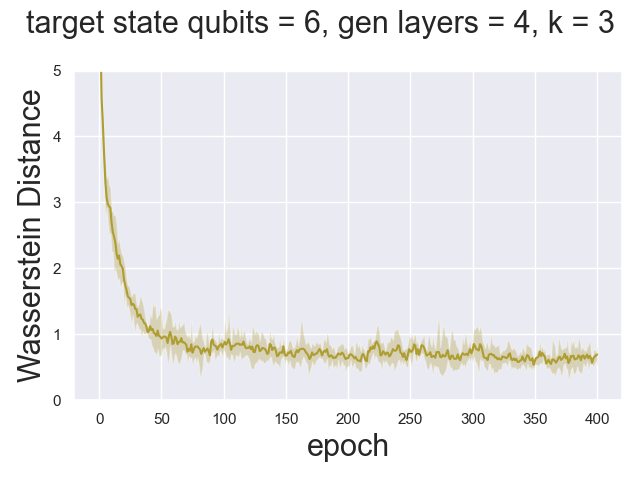
\includegraphics[width=0.3\linewidth]{figures/wqgans_phase_size=6_k=3_gen=4/Wasserstein_Distance.png}
  }
  \subfloat{
    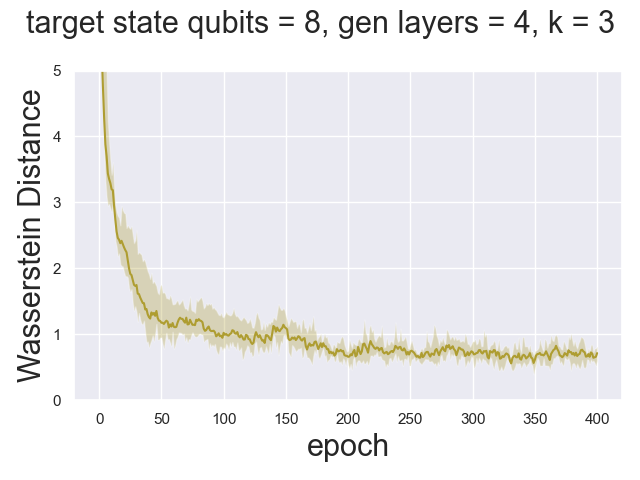
\includegraphics[width=0.3\linewidth]{figures/wqgans_phase_size=8_k=3_gen=4/Wasserstein_Distance.png}
  }

  \subfloat{
    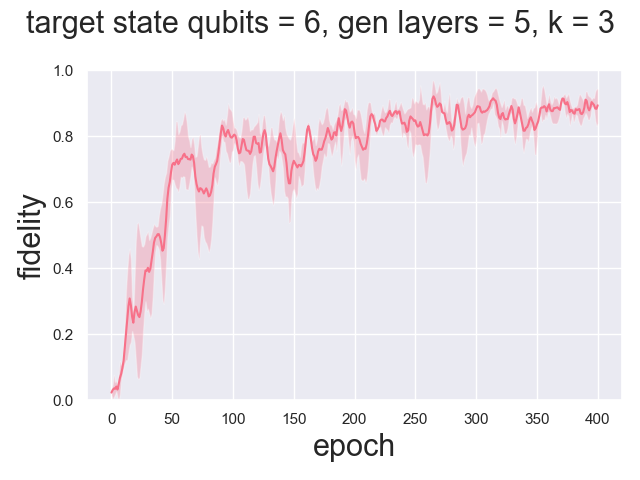
\includegraphics[width=0.3\linewidth]{figures/wqgans_phase_size=6_k=3_gen=5/fidelity.png}
  }
  \subfloat{
    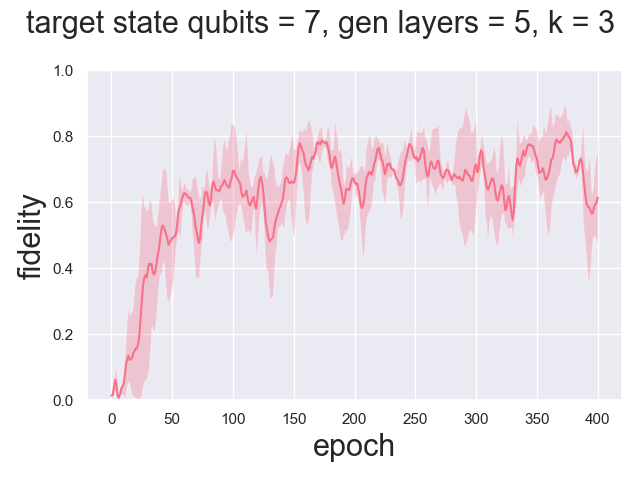
\includegraphics[width=0.3\linewidth]{figures/wqgans_phase_size=7_k=3_gen=5/fidelity.png}
  }
  \subfloat{
    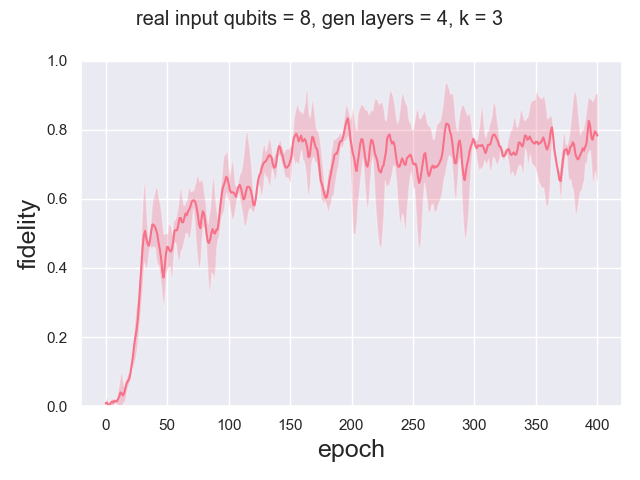
\includegraphics[width=0.3\linewidth]{figures/wqgans_phase_size=8_k=3_gen=5/fidelity.png}
  }

  \subfloat{
    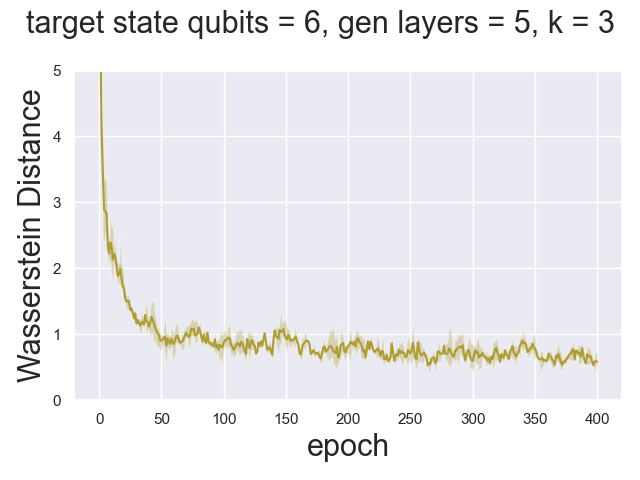
\includegraphics[width=0.3\linewidth]{figures/wqgans_phase_size=6_k=3_gen=5/Wasserstein_Distance.png}
  }
  \subfloat{
    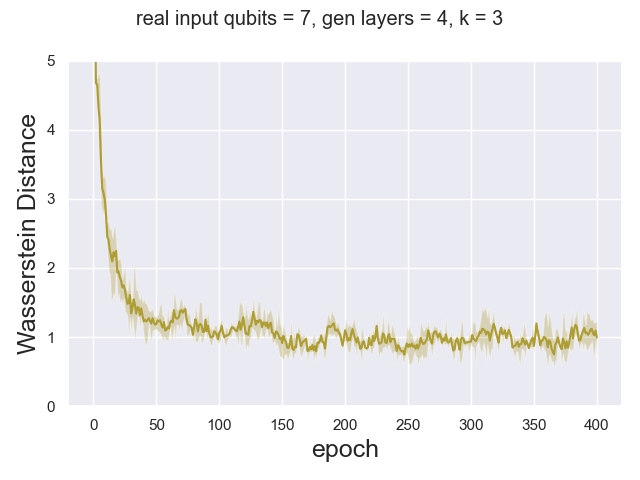
\includegraphics[width=0.3\linewidth]{figures/wqgans_phase_size=7_k=3_gen=5/Wasserstein_Distance.png}
  }
  \subfloat{
    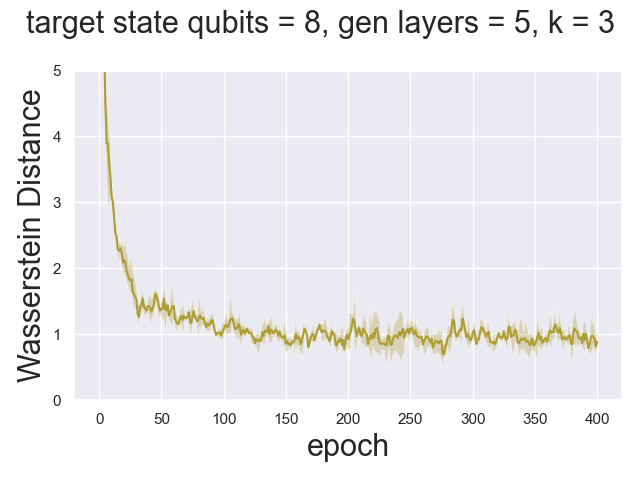
\includegraphics[width=0.3\linewidth]{figures/wqgans_phase_size=8_k=3_gen=5/Wasserstein_Distance.png}
  }
  \caption{Results of topological phase transition estimation (ansatz Appendix \ref{apx:topological_phase_transition_ansatz}).
    The solid line represents the average value and the shaded area
    represents the range from 5 different experiments. First the
    fidelity is shown and below the corresponding Wasserstein distance. In all the
    experiments the generator is built using ansatz from \ref{apx:sqgans_ansatz}.}
  \label{fig:wqgans_phase_res_3}
\end{figure}


\begin{figure}[htbp!]
  \captionsetup[subfigure]{labelformat=empty}
  \centering
  \subfloat{
    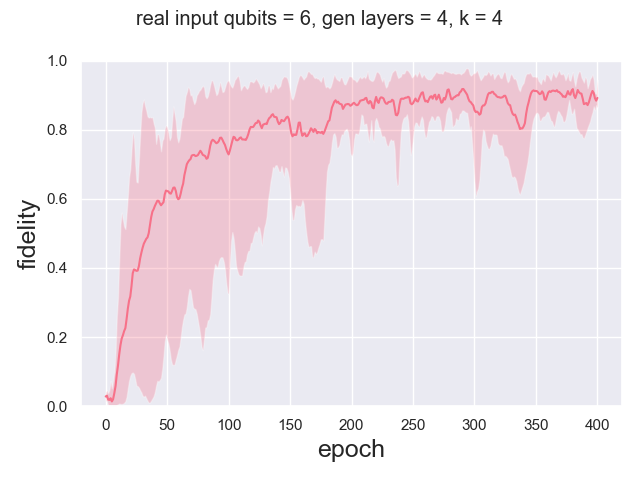
\includegraphics[width=0.3\linewidth]{figures/wqgans_phase_size=6_k=4_gen=4/fidelity.png}
  }
  \subfloat{
    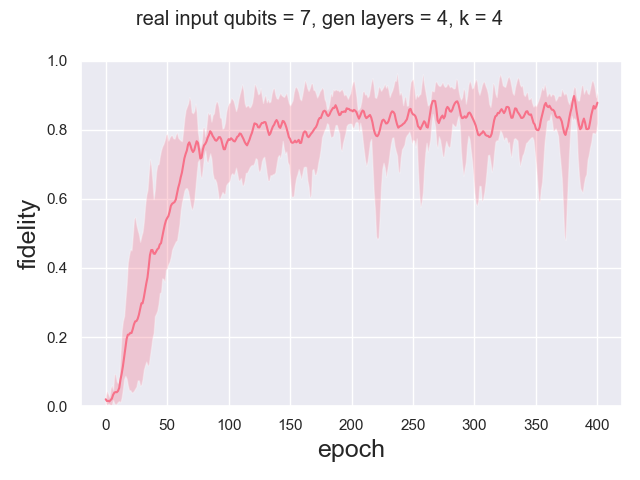
\includegraphics[width=0.3\linewidth]{figures/wqgans_phase_size=7_k=4_gen=4/fidelity.png}
  }
  \subfloat{
    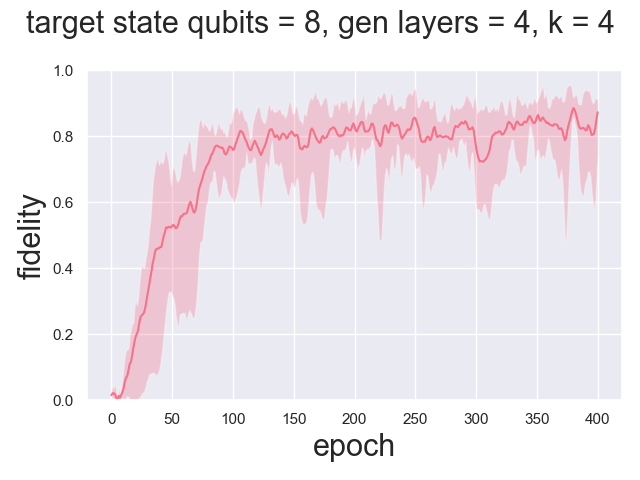
\includegraphics[width=0.3\linewidth]{figures/wqgans_phase_size=8_k=4_gen=4/fidelity.png}
  }

  \subfloat{
    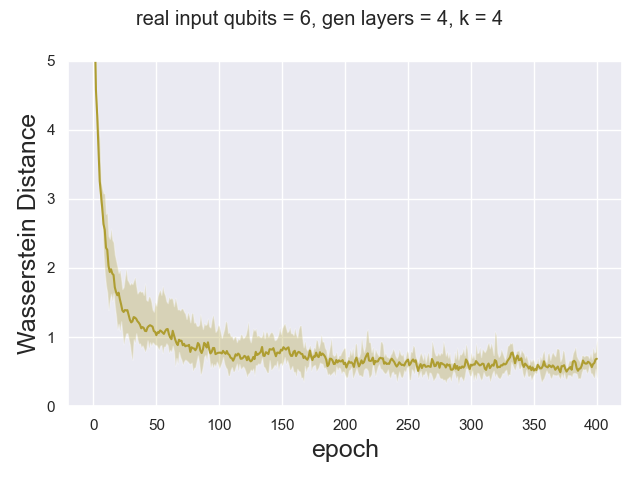
\includegraphics[width=0.3\linewidth]{figures/wqgans_phase_size=6_k=4_gen=4/Wasserstein_Distance.png}
  }
  \subfloat{
    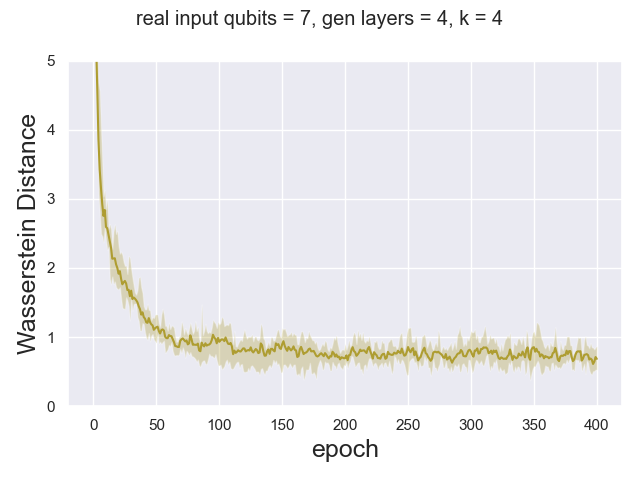
\includegraphics[width=0.3\linewidth]{figures/wqgans_phase_size=7_k=4_gen=4/Wasserstein_Distance.png}
  }
  \subfloat{
    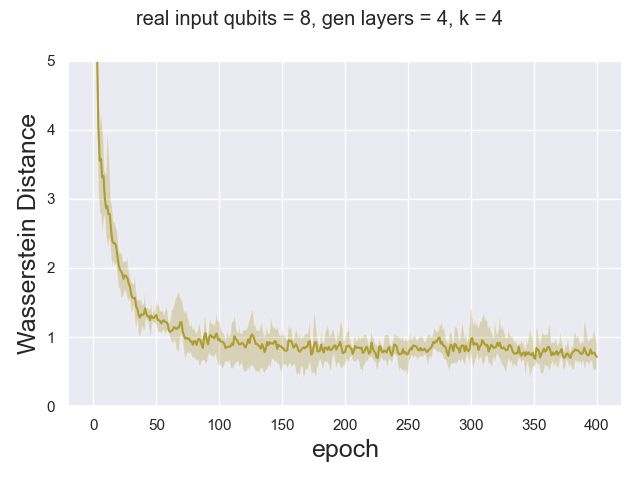
\includegraphics[width=0.3\linewidth]{figures/wqgans_phase_size=8_k=4_gen=4/Wasserstein_Distance.png}
  }
  
  \subfloat{
    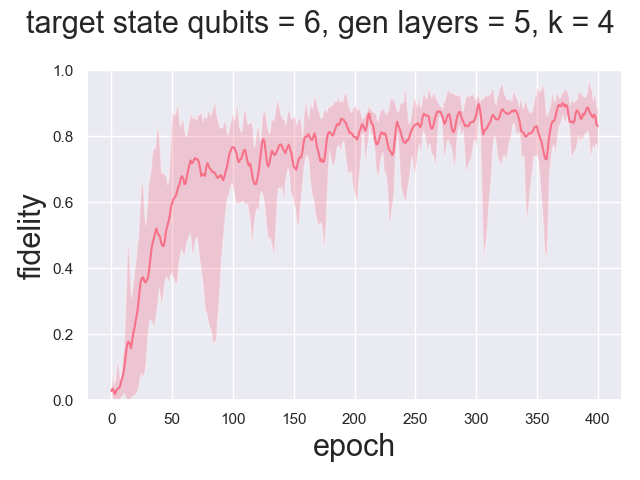
\includegraphics[width=0.3\linewidth]{figures/wqgans_phase_size=6_k=4_gen=5/fidelity.png}
  }
  \subfloat{
    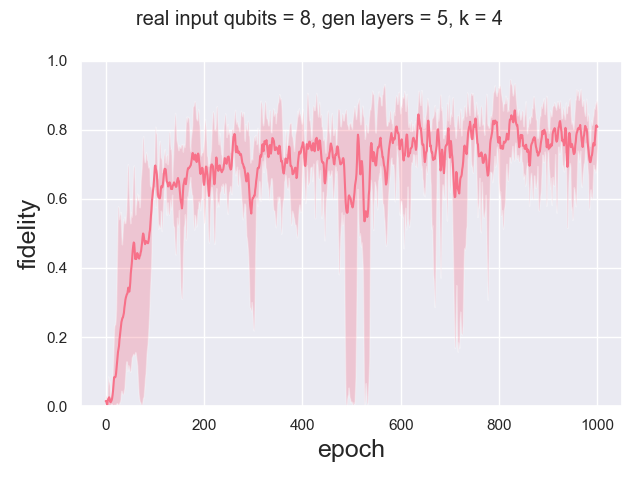
\includegraphics[width=0.3\linewidth]{figures/wqgans_phase_size=8_k=4_gen=5/fidelity.png}
  }
  \subfloat{
    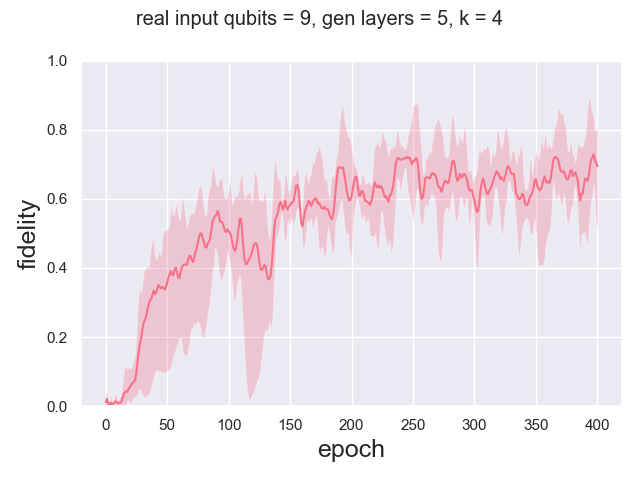
\includegraphics[width=0.3\linewidth]{figures/wqgans_phase_size=9_k=4_gen=5/fidelity.png}
  }

  \subfloat{
    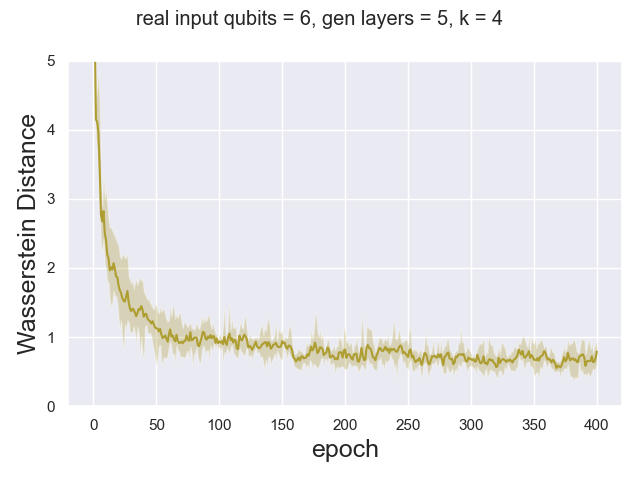
\includegraphics[width=0.3\linewidth]{figures/wqgans_phase_size=6_k=4_gen=5/Wasserstein_Distance.png}
  }
  \subfloat{
    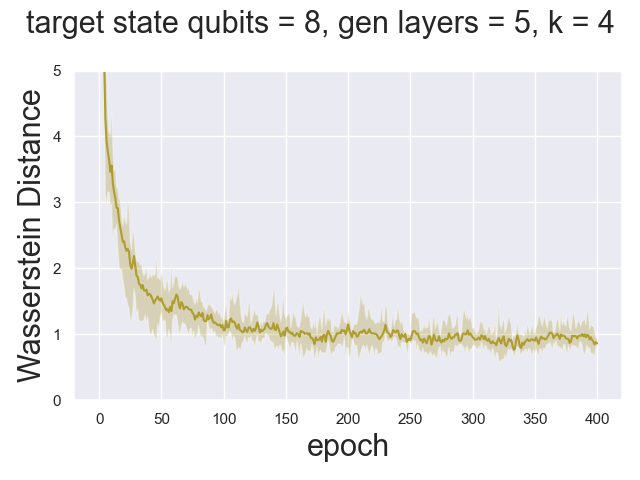
\includegraphics[width=0.3\linewidth]{figures/wqgans_phase_size=8_k=4_gen=5/Wasserstein_Distance.png}
  }
  \subfloat{
    \includegraphics[width=0.3\linewidth]{figures/wqgans_phase_size=9_k=4_gen=5/Wasserstein_Distance.png}
  }
  \caption{Results of topological phase transition estimation (ansatz Appendix \ref{apx:topological_phase_transition_ansatz}).
    The solid line represents the average value and the shaded area
    represents the range from 5 different experiments. First the
    fidelity is shown and below the corresponding Wasserstein distance. In all the
    experiments the generator is built using ansatz from \ref{apx:sqgans_ansatz}.}
  \label{fig:wqgans_phase_res_5}
\end{figure}
\label{apx:wqgans_pahse_results_butterfly}

\begin{figure}[htbp!]
  \captionsetup[subfigure]{labelformat=empty}
  \centering
  \subfloat{
    \includegraphics[width=0.25\linewidth]{figures/wqgans_butterfly_size=4_k=3_gen=4/fidelity.png}
  }
  \subfloat{
    \includegraphics[width=0.25\linewidth]{figures/wqgans_butterfly_size=5_k=3_gen=4/fidelity.png}
  }
  \subfloat{
    \includegraphics[width=0.25\linewidth]{figures/wqgans_butterfly_size=6_k=3_gen=4/fidelity.png}
  }
  \subfloat{
    \includegraphics[width=0.25\linewidth]{figures/wqgans_butterfly_size=7_k=3_gen=4/fidelity.png}
  }

  \subfloat{
    \includegraphics[width=0.25\linewidth]{figures/wqgans_butterfly_size=4_k=3_gen=4/Wasserstein_Distance.png}
  }
  \subfloat{
    \includegraphics[width=0.25\linewidth]{figures/wqgans_butterfly_size=5_k=3_gen=4/Wasserstein_Distance.png}
  }
  \subfloat{
    \includegraphics[width=0.25\linewidth]{figures/wqgans_butterfly_size=6_k=3_gen=4/Wasserstein_Distance.png}
  }
  \subfloat{
    \includegraphics[width=0.25\linewidth]{figures/wqgans_butterfly_size=7_k=3_gen=4/Wasserstein_Distance.png}
  }

  \subfloat{
    \includegraphics[width=0.25\linewidth]{figures/wqgans_butterfly_size=5_k=4_gen=4/fidelity.png}
  }
  \subfloat{
    \includegraphics[width=0.25\linewidth]{figures/wqgans_butterfly_size=6_k=4_gen=4/fidelity.png}
  }
  \subfloat{
    \includegraphics[width=0.25\linewidth]{figures/wqgans_butterfly_size=7_k=4_gen=4/fidelity.png}
  }
  \subfloat{
    \includegraphics[width=0.25\linewidth]{figures/wqgans_butterfly_size=8_k=4_gen=4/fidelity.png}
  }

  \subfloat{
    \includegraphics[width=0.25\linewidth]{figures/wqgans_butterfly_size=5_k=4_gen=4/Wasserstein_Distance.png}
  }
  \subfloat{
    \includegraphics[width=0.25\linewidth]{figures/wqgans_butterfly_size=6_k=4_gen=4/Wasserstein_Distance.png}
  }
  \subfloat{
    \includegraphics[width=0.25\linewidth]{figures/wqgans_butterfly_size=7_k=4_gen=4/Wasserstein_Distance.png}
  }
  \subfloat{
    \includegraphics[width=0.25\linewidth]{figures/wqgans_butterfly_size=8_k=4_gen=4/Wasserstein_Distance.png}
  }
  \caption{Results of butterfly circuit estimation (ansatz Appendix \ref{apx:butterfly_ansatz}).
    The solid line represents the average value and the shaded area
    represents the range from 5 different experiments. First the
    fidelity is shown and below the corresponding Wasserstein distance. In all the
    experiments the generator is built using ansatz from \ref{apx:sqgans_ansatz}.}
  \label{fig:wqgans_res_butterfly_3}
\end{figure}
\let\clearpage\oldclearpage
\chapter{Code and Technologies}
All the code used for this work is available on public github repository:
\url{https://github.com/WiktorJ/quantum-gans}.

The quantum circuits were implemented using Cirq
\cite{https://doi.org/10.5281/zenodo.5138274} and evaluated using Tensorflow
Quantum \cite{broughton2020tensorflow}. The optimization of the classical and
quantum networks was performed using optimizers from Tensorflow library \cite{tensorflow2015-whitepaper}.

All the quantum circuits schematics were drawn using Quantikz \cite{https://doi.org/10.17637/rh.7000520}.


% \section{Example 1}
% \cmark
% \section{Example 2}
% \xmark

%%% Local Variables:
%%% mode: latex
%%% TeX-master: "../main"
%%% End:

\microtypesetup{protrusion=false}
\listoffigures{}
\listoftables{}
\microtypesetup{protrusion=true}
\printglossaries
\printbibliography{}

\end{document}
